\chapter{软件变更影响域分析}
\label{chap_impact}
如前所述,我们需要对补丁中的变更进行语义影响域分析,以此来找到变更对应的语义影响域,用于进行后续的冲突检测。

通过语义影响域分析,我们就可以从代码中挖掘出所需要的变更影响域信息,从而可以进行后续的冲突检测工作。

实际上,语义影响域分析主要分为两个子过程,即程序间差异分析和变更影响分析,通过这两个分析的协作来完成整个语义影响域的分析。

我们可以将整个语义影响域分析过程定义为如下的函数,该分析过程先将版本演进的过程转化为补丁,再去计算补丁对程序代码的语义影响域:

\begin{definition}
	$ia: Code \times Code \mapsto {Structure}$。$s = ia(v_i,v_j) = impact(diff(v_i,v_j),v_i),i,j \subset \mathbb{N}$。
\end{definition}

因此,整个语义影响域分析过程可以用算法\ref {algo_impact}描述。

在兼容性检测工具中,该部分工作被实现为影响域分析模块,该模块需要对$ia$函数进行实际的实现。因此,该模块可以对应地拆分为两个子模块分别进行实现:
\begin{itemize}
	\item 差异性分析模块:实现相应的程序差异性分析过程。即$diff$函数的实现。
	\item 影响分析模块:实现相应的变更影响分析过程。即$impact$函数的实现。
\end{itemize}

该模块中首先需要定义好合适的影响范围和影响元素的级别。

事实上,可以将程序中受变更影响的部分划分为不同的粒度,从而获得不同程度的影响\cite{petrenko2009variable},我们考虑对面向对象的编程方法中的影响元素级别进行划分:

\begin{enumerate}
	\item 类:探讨变更对于其他类和对象的影响。对于面向对象的程序设计方法而言,这是最高级别的粒度。
	\item 方法:探讨变更对于其他方法的的影响。
	\item 基本块:探讨变更对于其他基本块的影响。
	\item 语句:探讨变更对于其他语句的影响。
\end{enumerate}

而所谓的影响范围也需要界定其粒度,不同层级的粒度显然会对语义影响域分析的精度产生影响。

\begin{enumerate}
	\item 类间:考虑变更的影响可能延伸到其他类、对象。
	\item 方法间:考虑变更的影响可能延伸到其他方法内部。
	\item 方法内部:考虑变更的影响只在本方法的内部延伸。
\end{enumerate}

不同级别的影响范围均可分别采用不同的影响元素级别。

在实际情况中,我们主要采用了较为简单的分析过程,即将影响范围限制在方法内部,但是将受影响元素设置为程序语句级别,以保证精度。

在实现该模块的过程中,由于我们可以采用现有工具来完成具体的程序间差异分析和变更影响分析过程,因而这两个子过程的分析算法可以直接使用已有的成熟算法。我们可以将主要精力放在如何整合两个子过程,并将其工具实现进行改进,以适用于兼容性检测问题的具体情况。

下面分别对这两个子过程的分析方法和对应模块的设计与实现进行叙述。

\begin{algorithm}[H]
	\caption{语义影响域分析算法}
	\label{algo_impact}
	\begin{algorithmic}[1]
		\Require $v_i$,$v_j$,即两个不同版本的代码	
		\Ensure $s$,即版本间的变更对于版本$v_i$的语义影响域
		\Function {ia}{$v_i,v_j$}
		\State $p \gets diff(v_i,v_j)$
		\State $s \gets impact(p,v_i)$
		\State\Return{$s$}
		\EndFunction
	\end{algorithmic}
\end{algorithm}

\section{程序间差异性分析}
\label {chap_diff}

程序间差异性分析是$diff$函数的实现。它主要用于分析两个不同版本的程序之间的差异性,其结果即我们所需要的程序变更集合。

近年来程序间差异性分析方面有不少工作,实现了一些较为成熟的比较工具,我们可以使用这些工具来实现其所对应的差异性分析子模块。

\subsection{分析方法}

在本文的组合架构中,程序间差异性分析的主要任务是接受两个不同版本的源代码,并返回代码间的结构化差异信息。结构化的差异信息可以视为补丁的一种,只不过它具有比常见的采用Unix diff工具生成的$.patch$类型的补丁文件更丰富的信息,能够描述以程序语法结构的形式对软件变更进行描述。

该分析过程应该满足如下需要:
\begin{itemize}
	\item 输入为两个不同版本的代码。
	\item 输出为源代码间的软件变更集合。
	\item 每条变更描述语句或基本块级别的变更。
	\item 每条变更描述新旧程序结构的相关信息和其关联关系。
	\item 每条变更描述了其所属的作用域。
\end{itemize}

选择这样的分析结果类型是为了后续分析过程的方便,因为变更影响分析需要我们提供软件变更集合作为输入,而$.patch$类型的补丁文件只描述文本行的变更,不包含语法信息,我们无法从中提取出所需的语法层面的变更信息。

一种比较好的选择是采用抽象语法树AST(Abstract Syntax Tree)差异性分析,因为抽象语法树中包括了足够多的语法结构信息。

\subsection{模块设计与实现}

本文中主要采用jpf-regression工具自带的前置工具ASTro来实现差异性分析模块的功能。该子模块实现了$diff$函数的实际功能,接受两个不同版本的Java源代码文件作为输入,以XML格式输出程序间的变更集合。

\subsubsection{设计}

在该模块的设计中,其输入输出过程可以描述如图\ref {differ},输入输出的具体描述参见表\ref {differ_io}。

\begin{figure}[H]
	\centering
	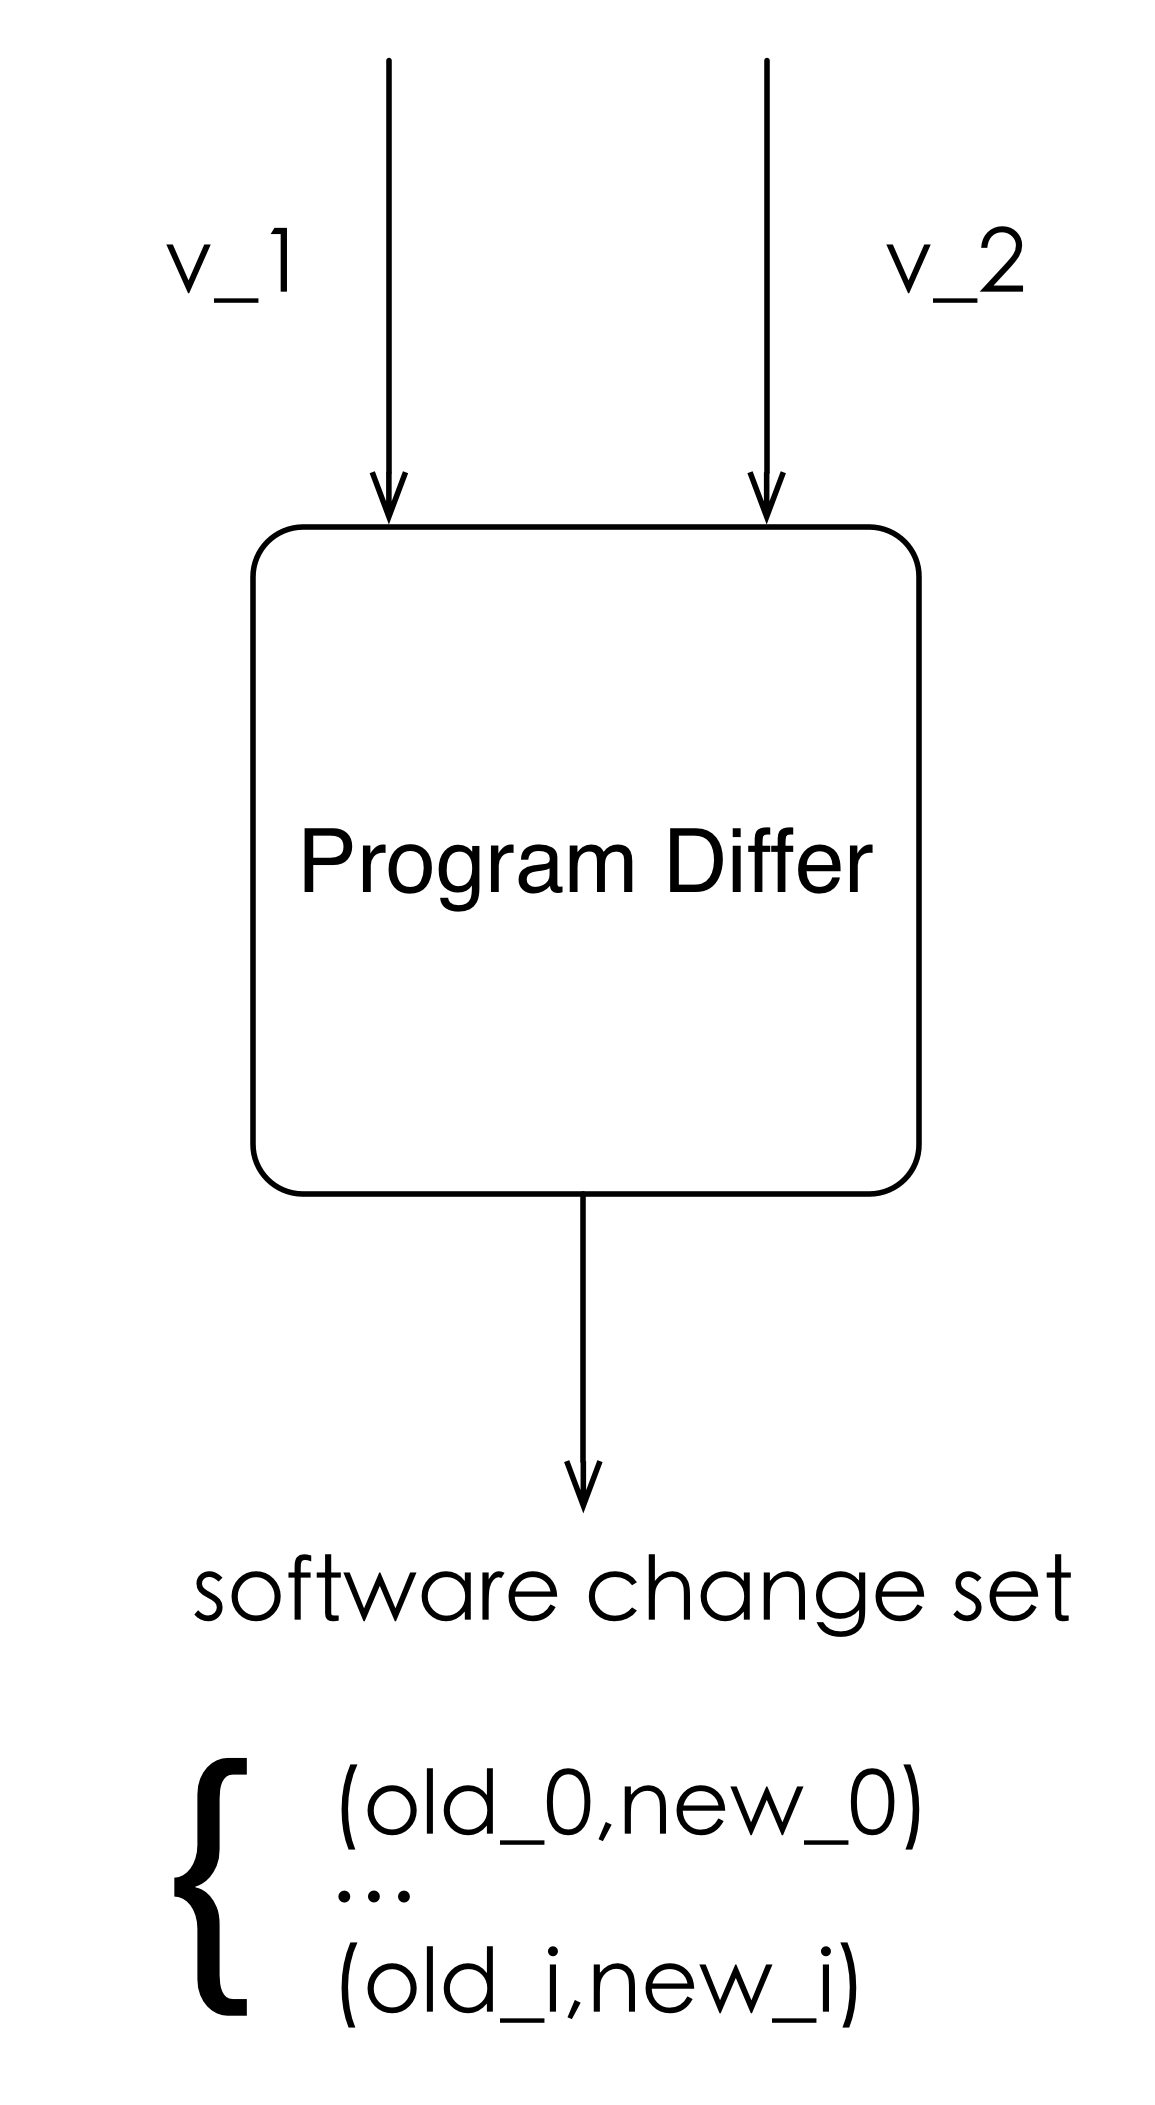
\includegraphics[height=.6\columnwidth]{chap03_differ}
	\caption {差异性分析模块}
	\label {differ}	
\end{figure}

图中所描述的模块输出——软件变更集合,设计为如下的格式,即变更前后的代码结构所组成的二元组集合:
\begin{definition}
	$ change\_set = \{ (old_i,new_i) \mid  old_i \subset Structure,new_i \subset Structure, i \subset \mathbb{N} \}$
\end{definition}

由于该模块需要调用其他工具来完成具体的差异性分析过程,其输出应作为影响分析模块的输入,可见该模块的核心任务包括:
\begin{itemize}
	\item 差异性分析
	\item 输入输出
\end{itemize}

因此该模块的内部设计可以参考图\ref {des_diff}。

该模块的流程也就可以设计成如下的形式:
\begin{enumerate}
	\item 读取输入
	\item 进行差异性分析
	\item 输出分析结果
\end{enumerate}

\begin{figure}[H]
	\centering
	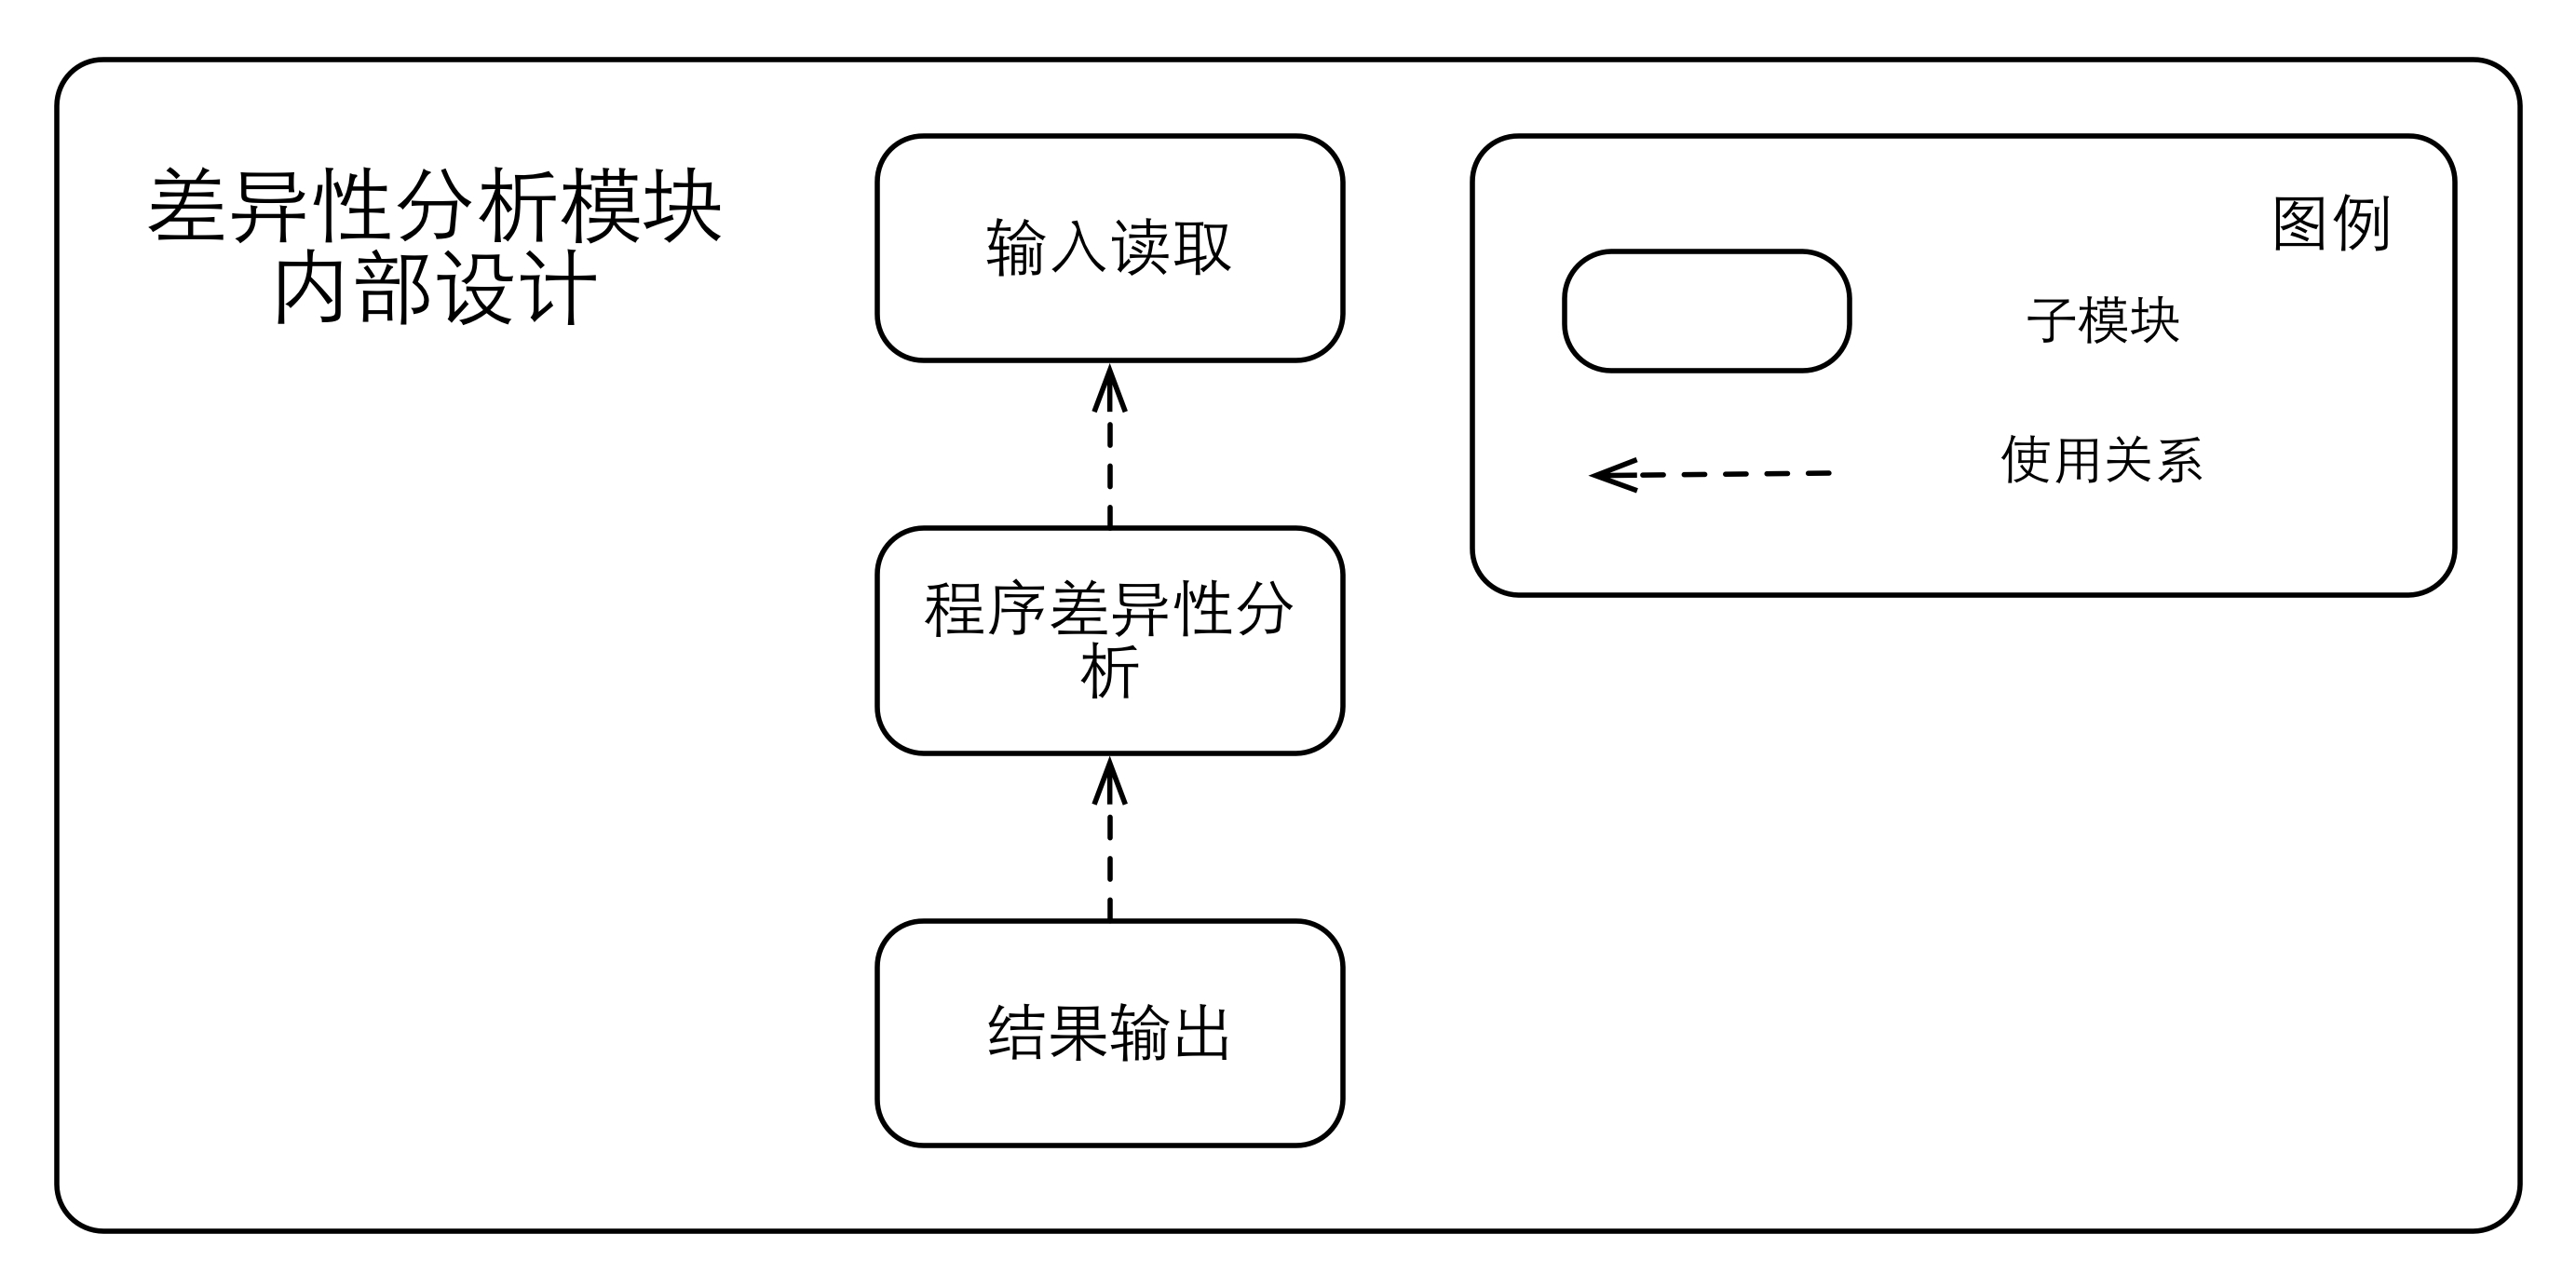
\includegraphics[width=.8\columnwidth]{chap04_diff_des}
	\caption {模块设计}
	\label {des_diff}	
\end{figure}


\begin{table}
	\caption{输入输出对照表}
	\label{differ_io}
	\centering
	\begin{tabular}{lc}
		\toprule[1.5pt]
		{\heiti 输入输出} & {\heiti 描述}\\\midrule[1pt]
		$v_1$ & 源代码 \\
		$v_2$ & 源代码 \\
		$change\_set$ & 变更集合 \\
		\bottomrule[1.5pt]
	\end{tabular}
\end{table}

\subsubsection{实现}

在该模块的实现过程中,采用了ASTro工具来完成具体的程序间差异分析过程。

因而实际上该模块的输入输出可以参考表\ref {differ_io2}。

\begin{table}[H]
	\caption{输入输出对照表}
	\label{differ_io2}
	\centering
	\begin{tabular}{llc}
		\toprule[1.5pt]
		{\heiti 输入输出} & {\heiti 描述} & {\heiti 格式}\\\midrule[1pt]
		输入 & 源代码 & Java\\
		输入 & 源代码 & Java\\
		输出 & 影响分析模块配置文件 & JPF\\
		输出 & 变更集合 & XML\\
		\bottomrule[1.5pt]
	\end{tabular}
\end{table}

ASTro支持对Java代码的比对。它会比对两个文件的抽象语法树,并从中抽取出对应的不同之处,形成语法结构上的差异性,并输出为XML格式的文件以供后续分析过程使用。

该工具输出的XML文件将源代码按照抽象语法树的格式进行输出,其节点级别为基本块,并提供了丰富的差异性信息,如两个版本代码的对应节点是否发生了变更等。

利用这些输出信息,我们可以从中提取出程序的变更集合,从而进行后续的变更影响分析。

在实际使用中,为了满足本文的需要,在将该工具整合进来时进行了一些改进。


受限于ASTro工具的具体实现,其输出结果的存在一定的问题,主要包括:
\begin{enumerate}
	\item 对某些代码文件无法完成差异性分析。
	\item 对某些代码文件输出结果不准确,存在过高估计(over-estimate)的问题。
\end{enumerate}

对于第一个问题,由于无法知道该工具的源代码,我们无法解决,不过这只是极少数现象。

对于第二个问题,我们分析其结果可以发现,其结果中存在误报的情况,即某些代码行并未发生变更,然而工具却报告其发生了诸如移动、先删后增之类的伪变更。同样由于无法知道该工具的源代码,我们无法从算法的角度进行修改,不过对于这样的情况,我们可以对其输出结果进行一定的预处理,将这些误报的情况进行过滤,保留一个真变更子集合即可。

预处理算法可以用伪代码\ref {xml}进行描述。

\begin{algorithm}
	\caption{XML结果过滤算法}
	\label{xml}
	\begin{algorithmic}[1]
		\Require $c_1 = diff(v_2, v_1), c_2 = diff(v_2,v_4)$
		\Ensure 过滤掉两个变更集合中的相同变更
		\State $del_1 \gets \varnothing$
		\State $del_2 \gets \varnothing$
		\For {$i = 0$ to $sizeof(c_1)$}
		\State $tc_1 \gets c_1[i]$
		\For {$j = 0$ to $sizeof(c_2)$}
		\State $tc_2 \gets c_2[j]$
		\If {$tc_1 == tc_2$}
		\State $del_1.add(tc_1)$
		\State $del_2.add(tc_2)$
		\EndIf	
		\EndFor
		\EndFor
		\State $c_1 \gets c_1.delete(del_1)$
		\State $c_2 \gets c_2.delete(del_2)$
	\end{algorithmic}
\end{algorithm}

我们可以归纳证明这种预处理操作的正确性。由于变更对于代码的影响是链式的,对于某次变更影响分析的结果集合$s_{i,j} = ia(v_i,v_j)$而言,假设对于其中任意一个受影响的元素$e_k$,其中$k \subset \mathbb{N}$,其影响来源可能包括如下几种可能:
\begin{enumerate}
	\item 其影响仅来源于变更$c_1$。
	\begin{itemize}
		\item 如果$c_1$为真变更,那么删除所有伪变更对于$e_k$没有影响。
		\item 如果$c_2$为伪变更,那么删除所有伪变更会导致$e_k$从集合$s_{i,j}$中被删除,但此时$e_k$本身即为伪影响,集合$s_{i,j}$的正确性会得到提高。
	\end{itemize}
	\item 其影响来源于多条变更$c_1,c_2\dots,c_m$,其中$m \subset \mathbb{N}$。
	\begin{itemize}
		\item 假若所有变更均为真变更,那么删除所有伪变更对于$e_k$没有影响。
		\item 假若来源变更集合中包括某几条伪变更,那么删除所有伪变更之后,仍然存在其他真变更,这些真变更仍然会在变更影响分析中导致$e_k$被添加到集合$s_{i,j}$中,因而也不会使集合$s_{i,j}$的正确性下降。
		\item 假若所有变更均为伪变更,那么删除所有伪变更会导致$e_k$从集合$s_{i,j}$中被删除,但此时$e_k$本身即为伪影响,集合$s_{i,j}$的正确性会得到提高。
	\end{itemize}
\end{enumerate}

可见,我们的预处理操作是正确的,它不会导致结果集合$s = ia(v_i,v_j)$的正确性降低。


在实现该模块的时候,采用了shell脚本来完成分析过程的自动化,使该模块能够循环地调用ASTro进行分析,从而是实现对整个软件系统的所有代码进行批量化处理。若需要修改该模块的输入信息,只需要修改脚本中对应的输入数据即可。在这部分工作中,脚本代码主要完成了以下任务:

\begin{itemize}
	\item 实验数据定位,包括Java源代码和编译后的Class文件等。
	\item 根据代码的存放路径,计算其对应Class文件的位置。
	\item 获取代码文件名,以确定本次分析的对象。
	\item 实验数据的依赖JAR包定位。
	\item 创建输出文件目录。
	\item 定义ASTro的输入参数,包括输入文件位置、输出文件位置、查找路径等。
	\item 调用ASTro进行单次分析。
\end{itemize}

其中ASTro工具的使用格式可参考如下,其具体各参数的定义参考表\ref {ASTro}。

\begin{lstlisting} [style=BashInputStyle]
ASTDiffer 3/27/2013
USAGE: java ASTDiffer -original <file>.java -modified <file>.java 
-dir <output folder>
OPTIONAL: -file <fileName> -ocp <classpath> -mcp <classpath> 
-oco <outputDir> -mco <outputDir> -cs -xml
\end{lstlisting}	

\begin{table}
	\caption{ASTro参数对照表}
	\label{ASTro}
	\centering
	\begin{tabular}{llc}
		\toprule[1.5pt] 
		{\heiti 参数名} & {\heiti 描述} & {\heiti 启用}\\\midrule[1pt]
		-file & 分析目标的名字 & 是 \\
		-dir & 输出路径 & 是 \\
		-ocp & 旧版本代码的Classpath & 是\\
		-mcp & 旧版本代码的Classpath & 是\\
		-original    & 旧版本代码的位置 & 是\\
		-modified   & 新版本代码的位置 & 是\\
		-xml   & 以XML格式输出结果 & 是\\
		-cs   & 以变更脚本(Change Script)格式输出结果 & 否\\
		-heu   & 以启发式的方式进行匹配 & 是\\
		\bottomrule[1.5pt]
	\end{tabular}	
\end{table}

其次,我们采用了shell脚本完成了对后续分析过程的支持,能够自动批量化创建影响分析模块所需的配置文件。配置文件为自定义的JPF格式,通过类似键值对的方式定义了各项属性的值。JPF文件的格式等来自于Java Path Finder框架的设计,是该框架运行所必须的配置文件。该配置文件的具体属性为自定义,可以参考表\ref {JPF_prop}所述。

\begin{table}
	\caption{JPF属性对照表}
	\label{JPF_prop}
	\centering
	\begin{tabular*}{\linewidth}{lp{10cm}}
		\toprule[1.5pt]
		{\heiti 属性名} & {\heiti 描述} \\\midrule[1pt]
		target & 分析的目标 \\
		sourcepath & 源代码路径\\
		rse.ASTResults & ASTro工具的输出文件位置\\
		rse.newClass & 新版本代码的Class文件位置\\
		rse.oldClass    & 旧版本代码的Class文件位置\\
		rse.dotFile   & jpf-regression工具的Dot格式输出文件位置\\
		\bottomrule[1.5pt]
	\end{tabular*}
\end{table}

在使用shell脚本调用ASTro工具进行分析和输出影响分析模块的配置文件时,考虑到实际使用中,我们需要将新版本$v_2$作为对比的基准,以获取一致的行号。因而在进行变更影响分析时,我们需要进行相应配置,使得:
\begin{itemize}
	\item $s_1 = impact(diff(v_2,v_1),v_2)$,求得变更集合$p_1 = diff(v_2,v_1)$对版本$v_2$的影响范围$s_1$。
	\item $s_2 = impact(diff(v_2,v_4),v_2)$,求得变更集合$p_3 = diff(v_2,v_4)$对版本$v_2$的影响范围$s_2$。
\end{itemize}

实际上,也就是说:
\begin{itemize}
	\item 补丁$p_1 = diff(v_2,v_1)$,即将版本$v_2$视为“旧版本”,将版本$v_1$视为“新版本”。
	\item 补丁$p_3 = diff(v_2,v_4)$,即将版本$v_2$视为“旧版本”,将新版本应用补丁后的版本$v_4$视为“新版本”。
\end{itemize}

在实际操作中,我们只需做这样的版本交换即可。

整个差异性分析模块的工作流程可以参考图\ref {diff}。

\begin{figure}[H]
	\centering
	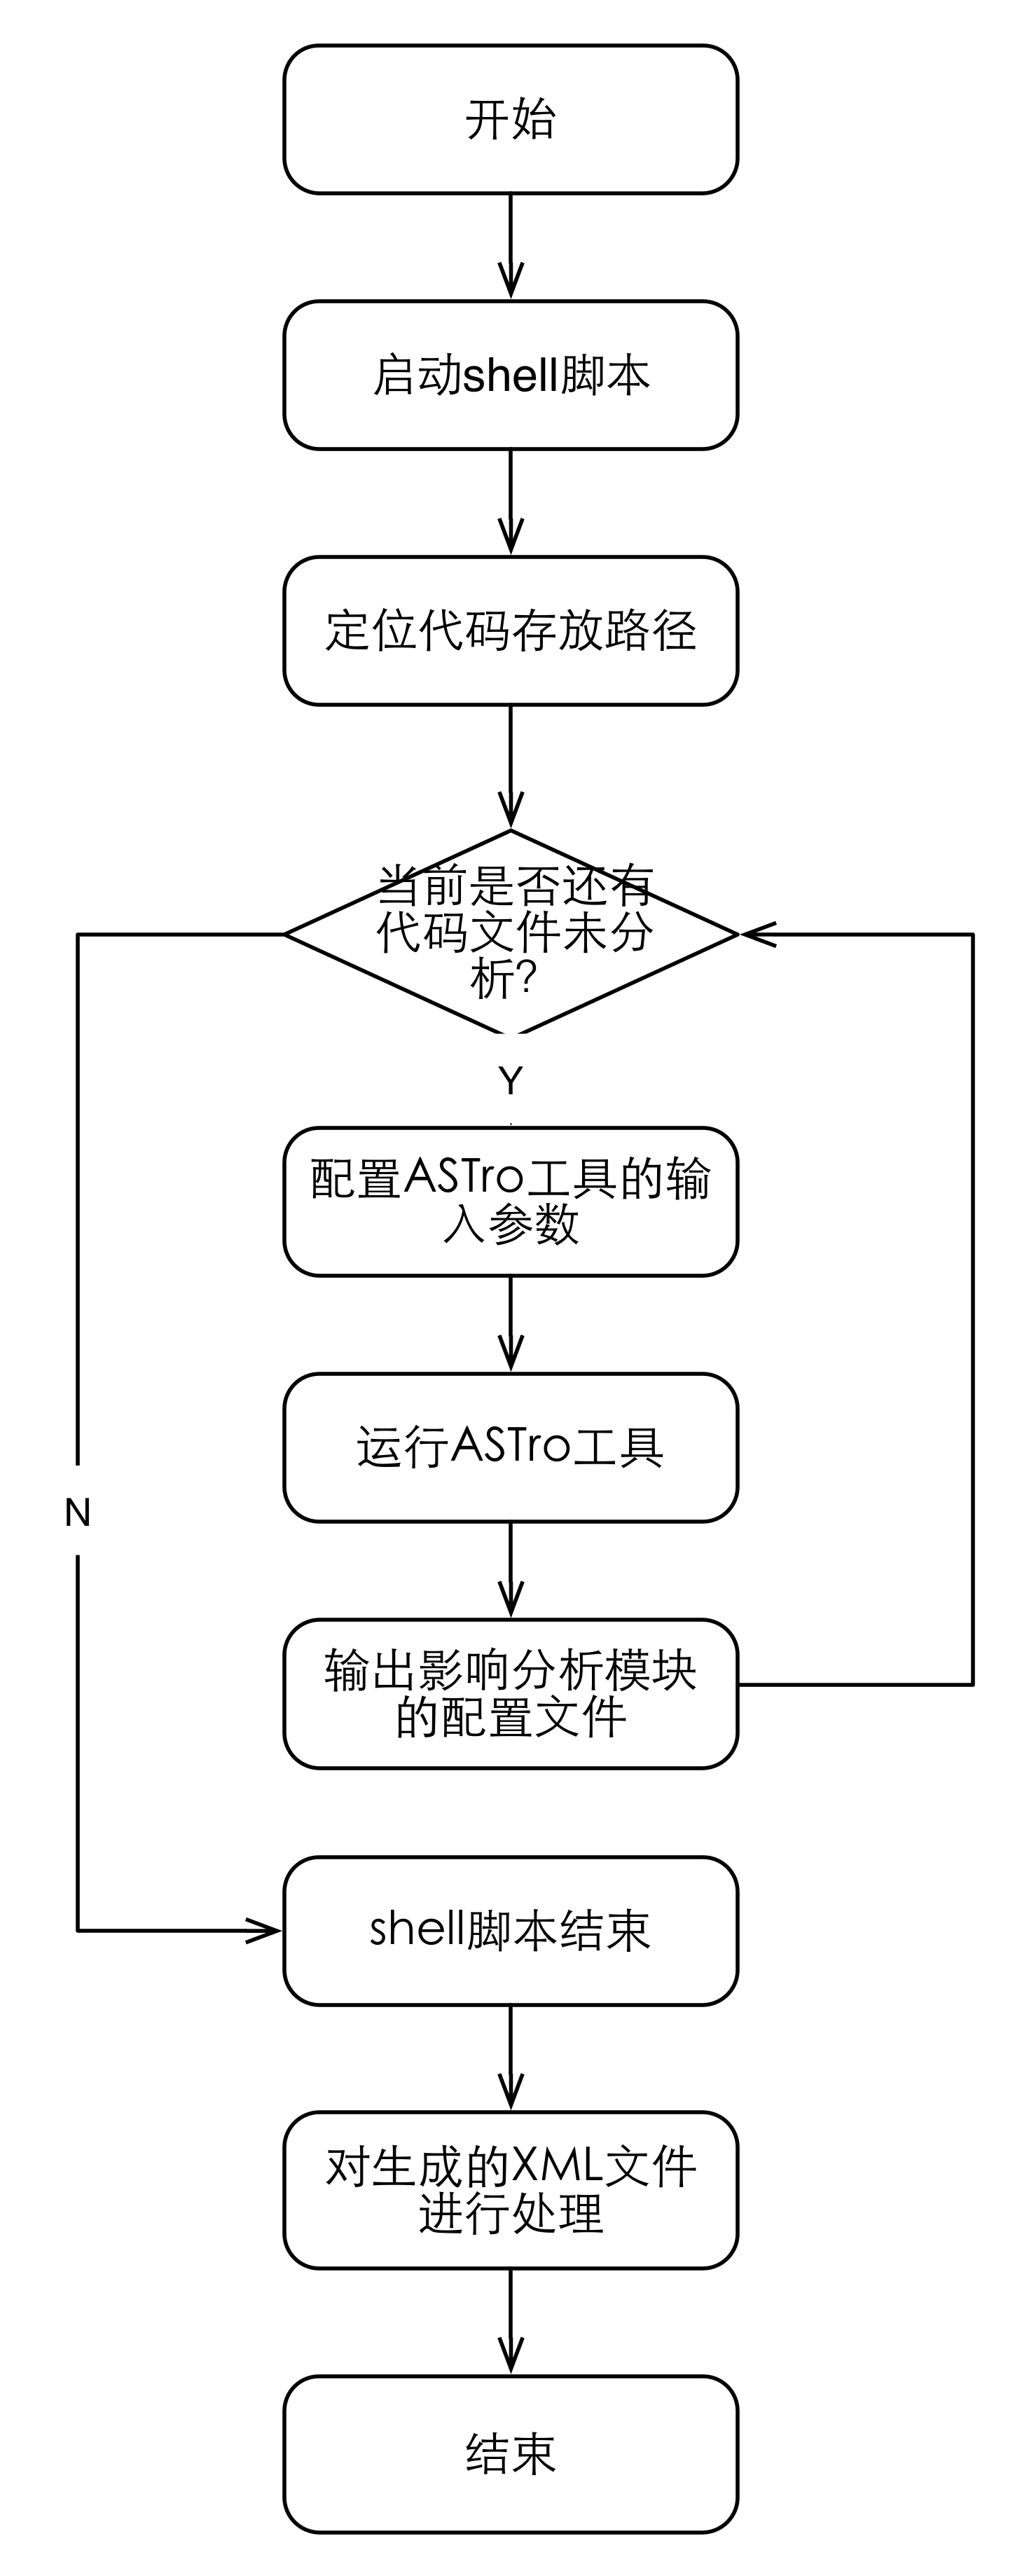
\includegraphics[height=.8\columnwidth]{chap04_differ}
	\caption {程序间差异性分析流程}
	\label {diff}	
\end{figure}



%图中所描述的软件变更集合可以定义如下:
%\begin{definition}
%	$ change\_set = \{ (old_i,new_i) \mid  old_i \subset Structure,new_i \subset Structure, i \subset \mathbb{N} \}$
%\end{definition}



\section{变更影响分析}
\label {chap_impact}

程序变更影响分析是$impact$函数的具体实现,主要用于获取变更集合对其他程序结构的影响域。影响域所包含的程序结构直接或间接地受到变更集合中的元素影响。

近年来这方面比较成熟的工作也有不少,因而可以直接选择合适的变更影响分析算法作为该过分析过程的具体实现。

\subsection{分析方法}

在本文的组合架构中,该分析过程应当接受两个不同版本代码间的变更集合作为输入,并输出变更集合所对应的影响集合,这也就是我们所需要的变更集合的语义影响域。变更影响分析的过程可以通过控制流、数据流等信息分析出变更集合中每条变更对其他程序结构是否存在影响,并进行闭包计算即可。

本文对于该分析过程的要求如下:
\begin{itemize}
	\item 接受两个不同版本代码间的变更集合作为输入。
	\item 计算得到该变更集合所对应的影响集合。
	\item 计算过程中可以指定受影响的范围和元素类型。
	\item 影响集合中的元素按照其不同类型进行分类。
	\item 具有影响追踪系统,将计算影响域的过程进行记录。方便后续的冲突分析过程进行回溯。
\end{itemize}

其中影响追踪系统可以定义成如下类型的函数。该函数接受一个影响域分析函数$ia(v_i,v_j)$,并返回对应的依赖关系集合。

\begin{definition}
	$impact\_track(ia(v_i,v_j)):(Code \times Code \mapsto {Structure}) \mapsto {depend}$
\end{definition}


%该分析过程如图\ref {impact_analyzer}所述,其中的$impact$函数可以任意选择某一能够满足上述要求的变更影响分析算法。
%
%图中所描述的变更影响集合可以定义如下:
%\begin{definition}
%	$impact\_set = \{ (structure_i) \mid  structure_i \subset Structure, i \subset \mathbb{N}\}$
%\end{definition}
%
%\begin{figure}[H]
%	\centering
%	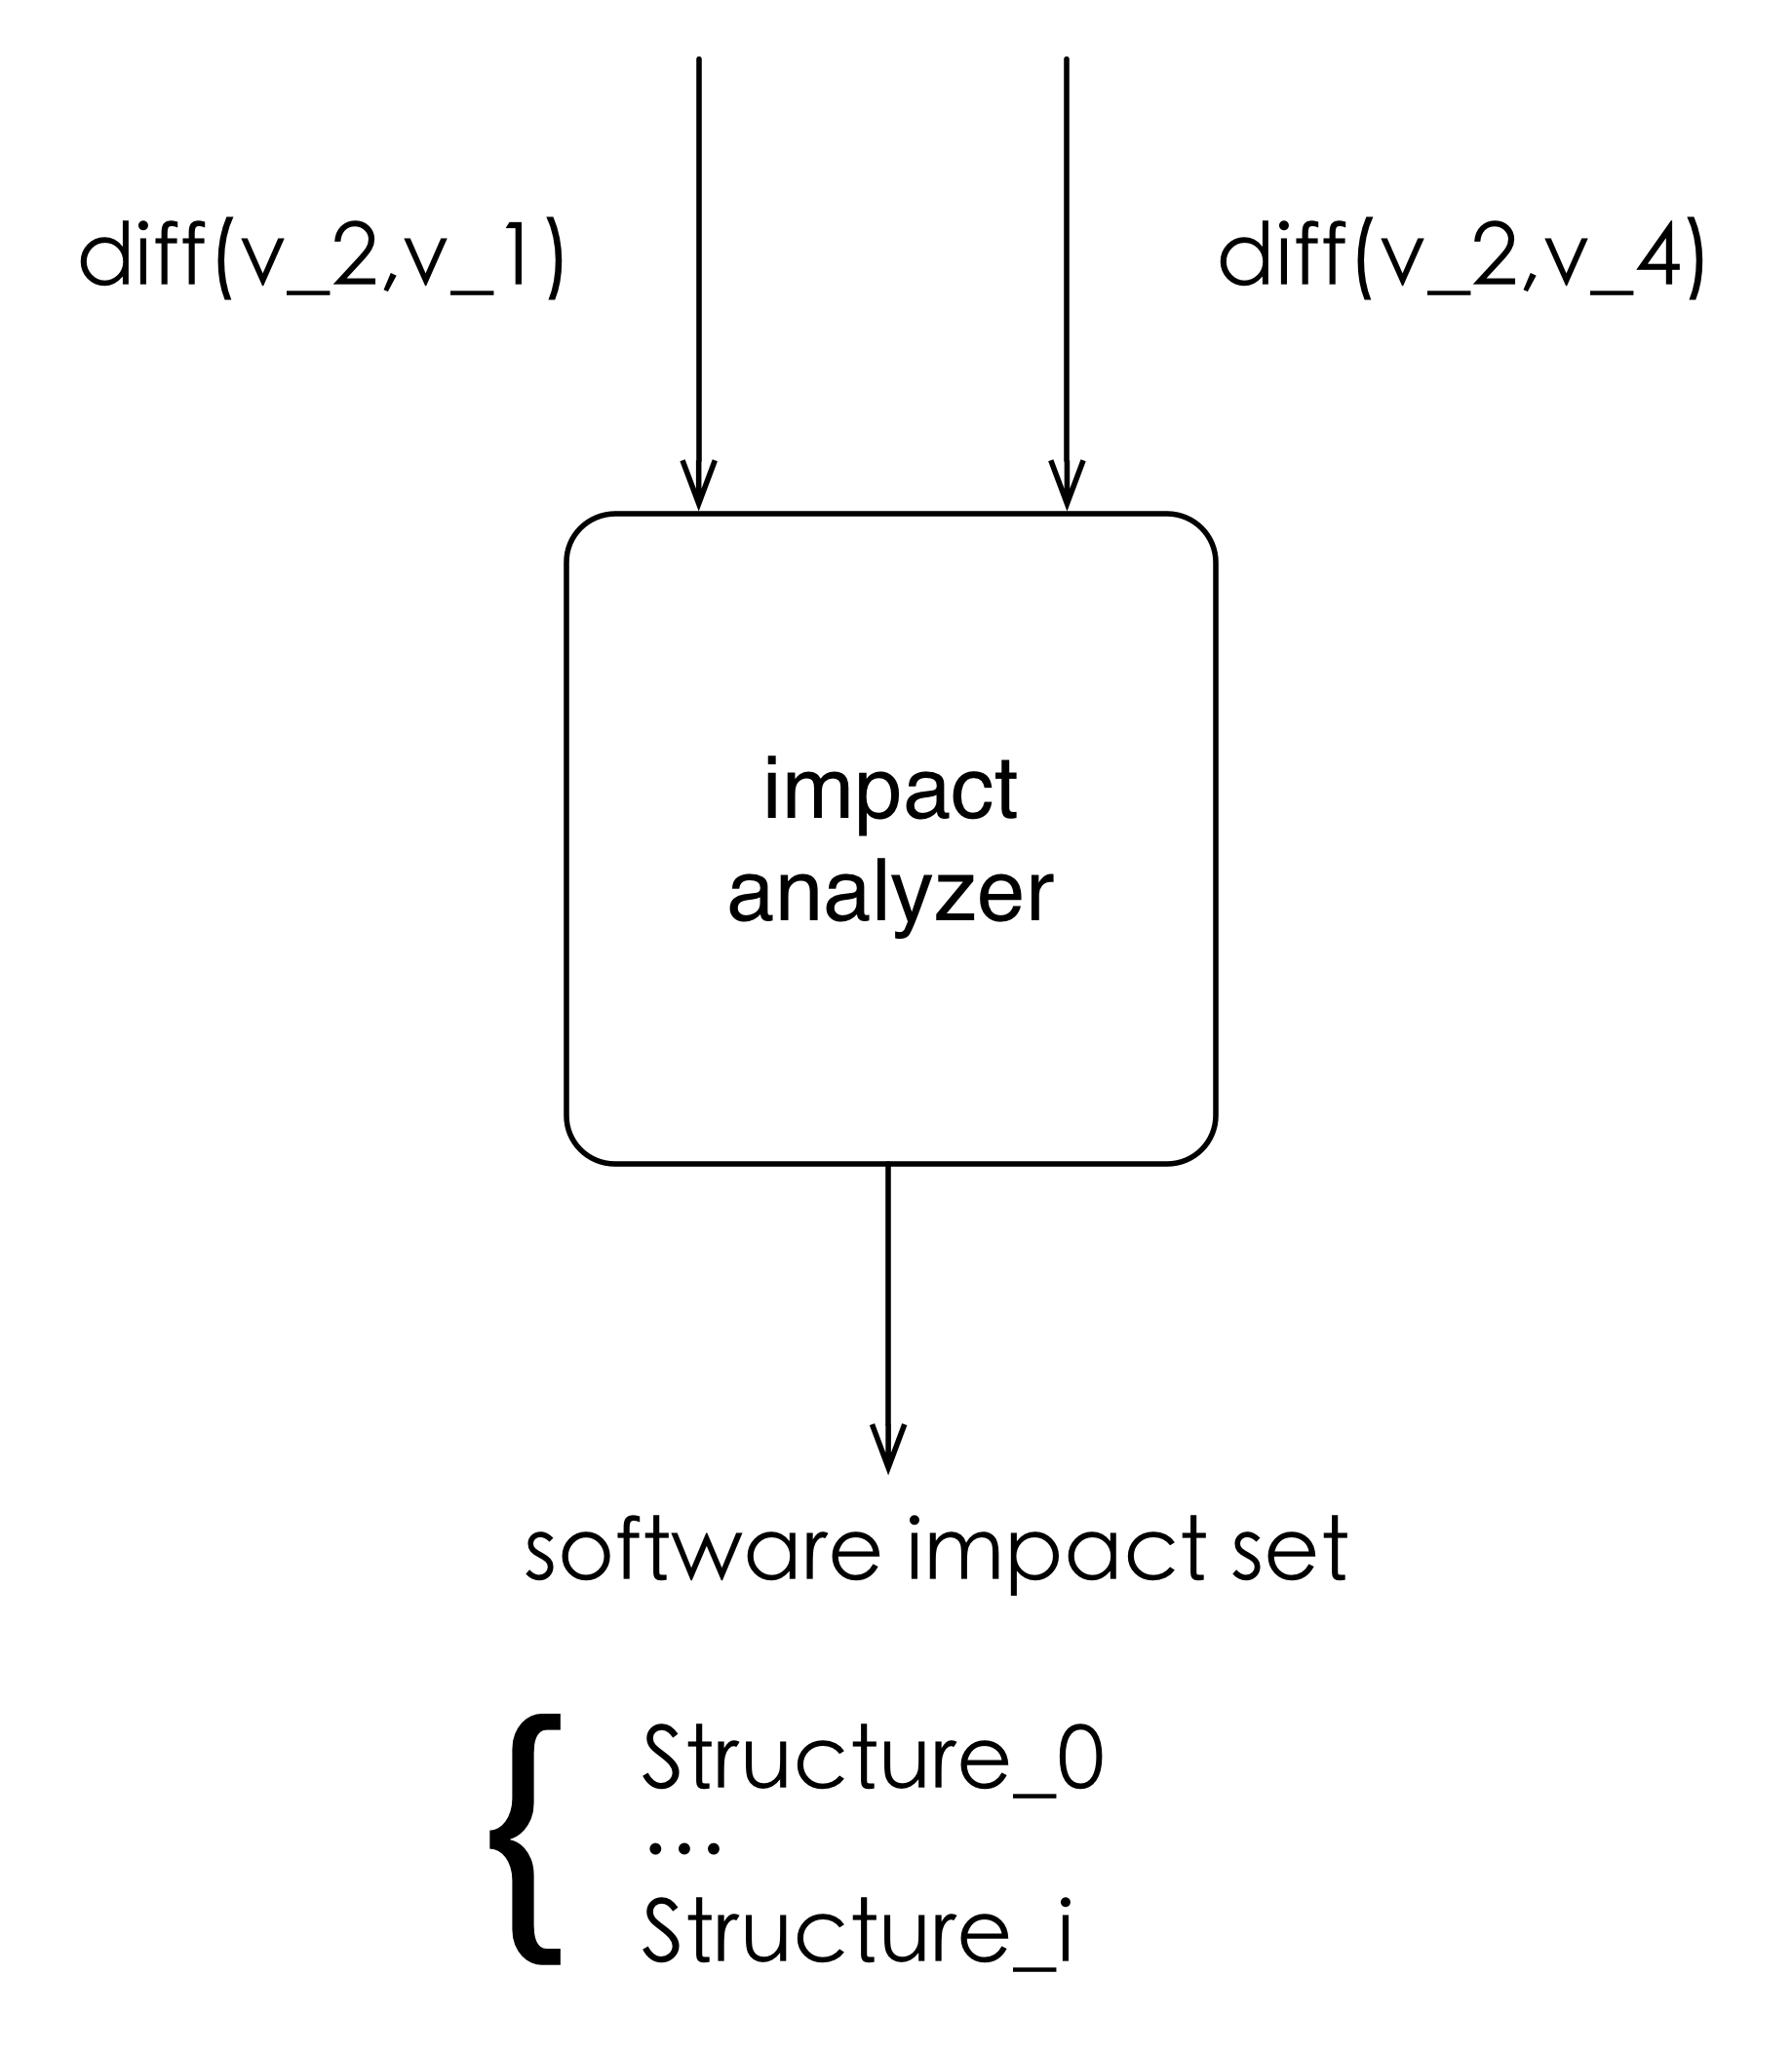
\includegraphics{chap03_impact}
%	\caption {程序间差异分析}
%	\label {impact_analyzer}	
%\end{figure}

\subsection{模块设计与实现}

本文中主要采用jpf-regression工具实现影响分析模块的功能。该子模块主要实现了$impact$函数的实际功能,它接受XML格式的变更集合作为输入,并输出Dot格式的影响域。

\subsubsection{设计}

在该模块的设计中,其输入输出过程可以描述如图\ref {impact},输入输出的具体描述参见表\ref {impact_io}。

考虑到该模块需要的核心任务包括:
\begin{itemize}
	\item 变更影响分析
	\item 影响追踪:记录影响分析过程的轨迹,即影响的依赖关系$depend$。
	\item 输入输出
\end{itemize}

因此,该模块的设计可以参考图\ref {des_impact}。

该模块的流程也就可以设计成如下的形式:
\begin{enumerate}
	\item 读取输入
	\item 变更影响分析,并进行影响追踪
	\item 结果输出
\end{enumerate}

\begin{figure}[H]
	\centering
	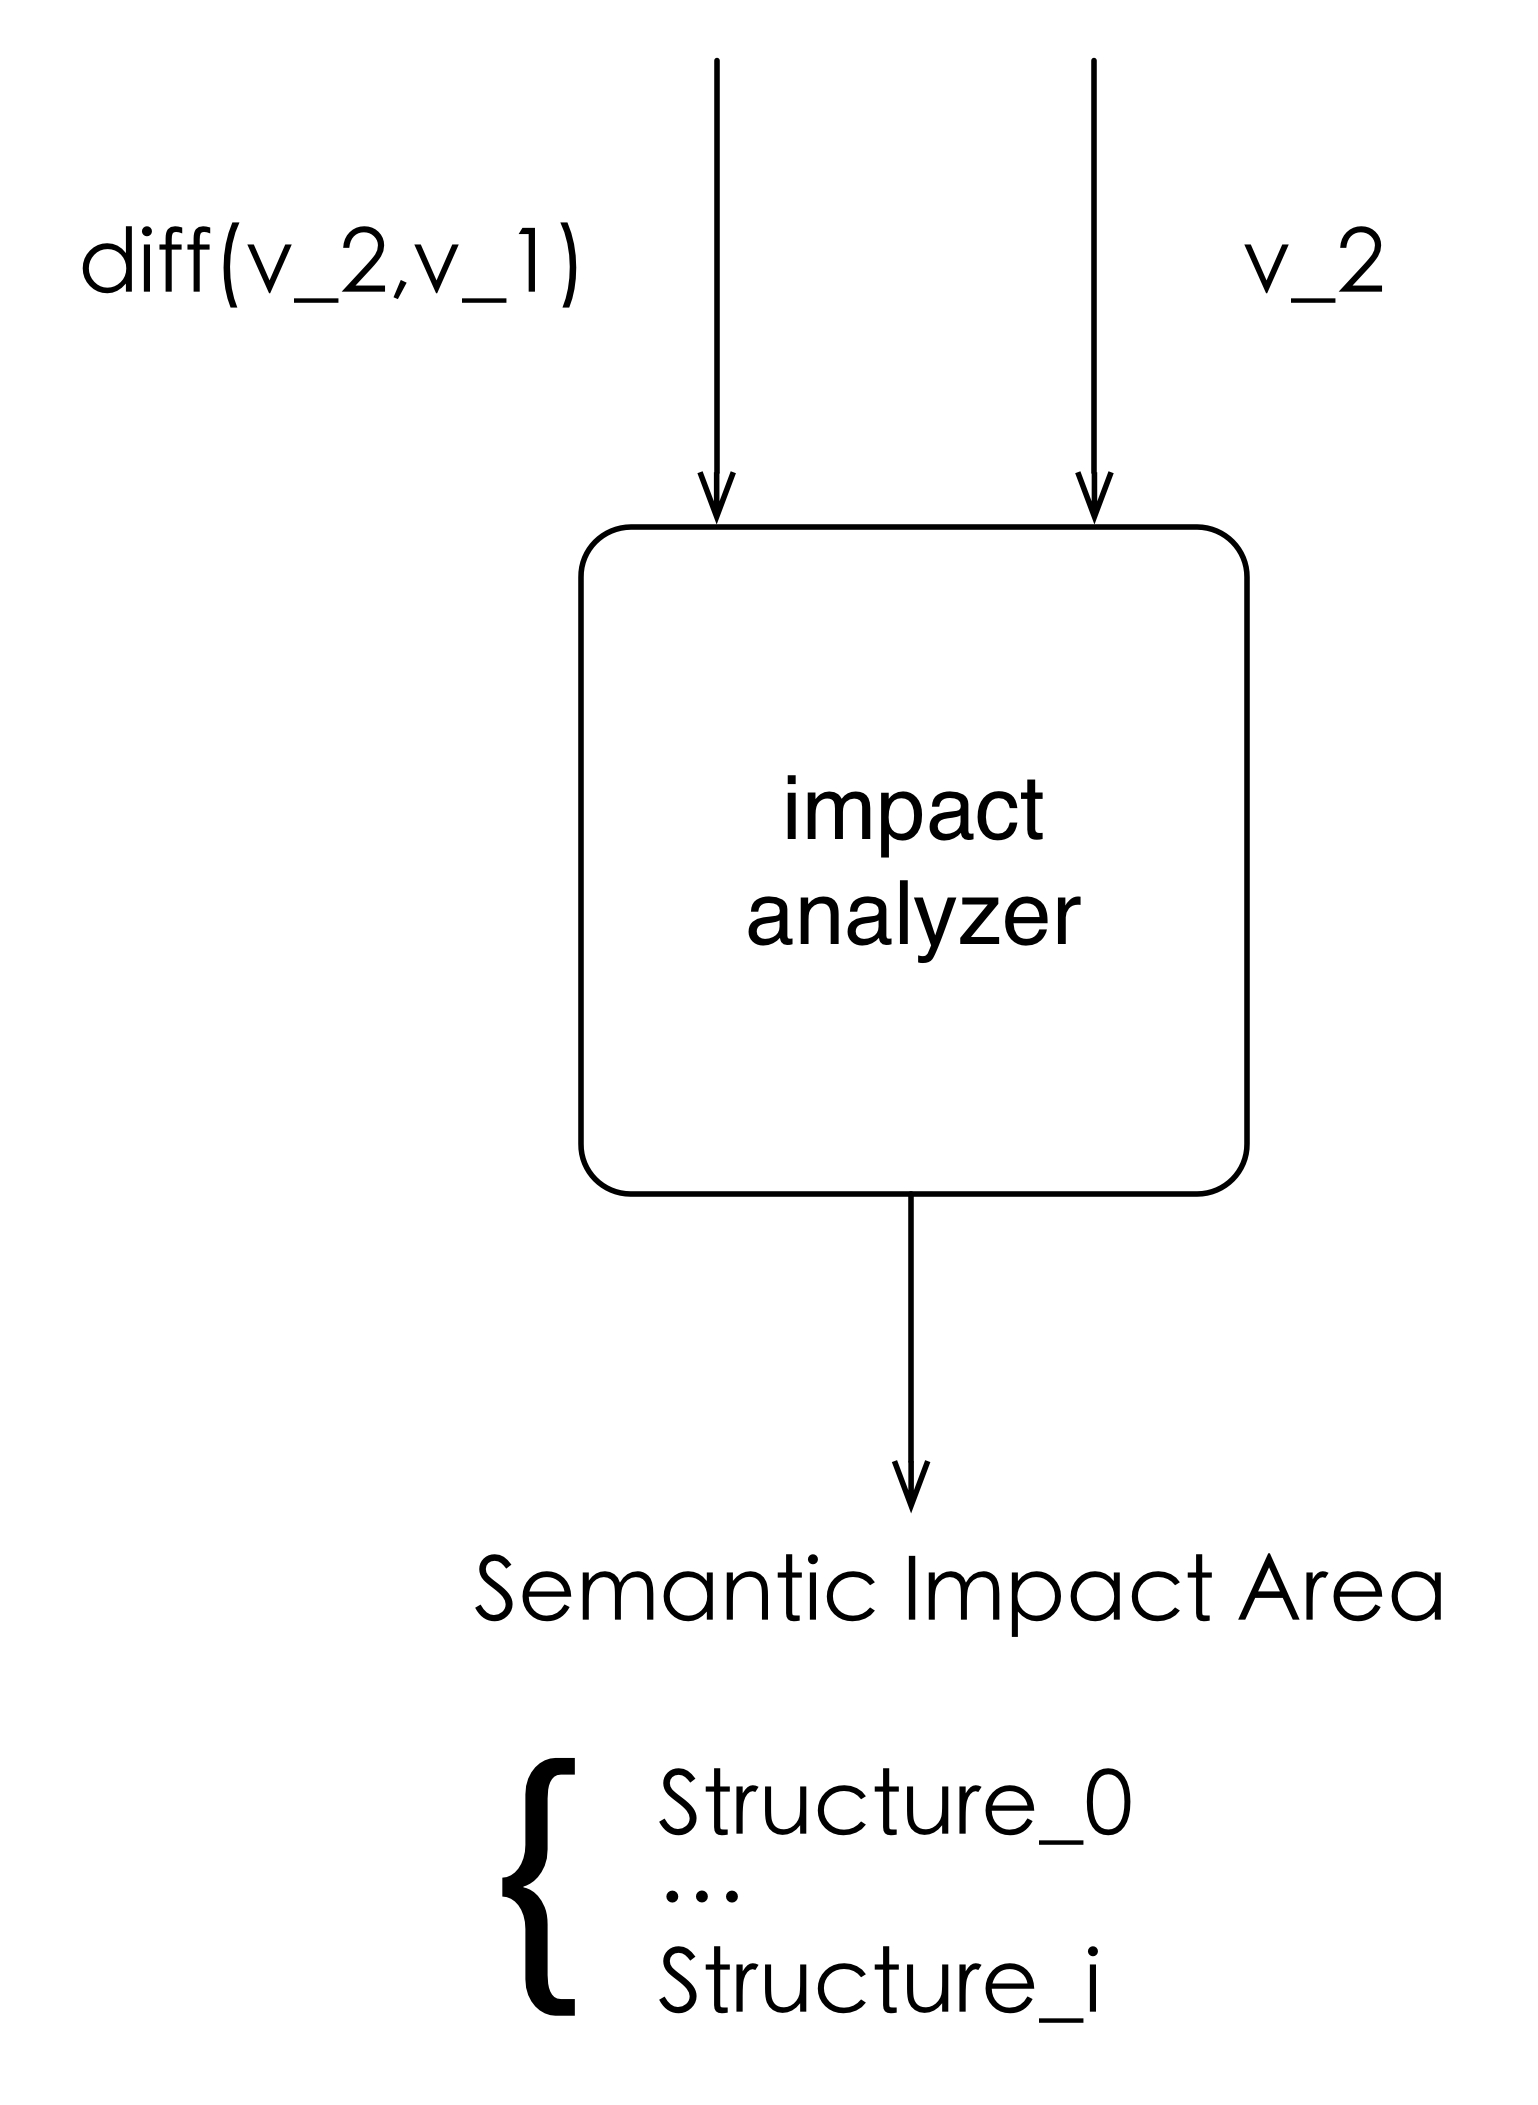
\includegraphics[height=.6\columnwidth]{chap03_impact2}
	\caption {影响分析模块}
	\label {impact}	
\end{figure}


\begin{table}[H]
	\caption{输入输出对照表}
	\label{impact_io}
	\centering
	\begin{tabular}{lc}
		\toprule[1.5pt]
		{\heiti 输入输出} & {\heiti 描述} \\\midrule[1pt]
		$diff(v_2,v_1)$ & 差异性分析模块的输出,变更集合 \\
		$v_2$ & 源代码 \\
		语义影响域 & 语义影响域,即$v_2$中受变更影响的代码结构集合\\
		\bottomrule[1.5pt]
	\end{tabular}
\end{table}

\begin{figure}[H]
	\centering
	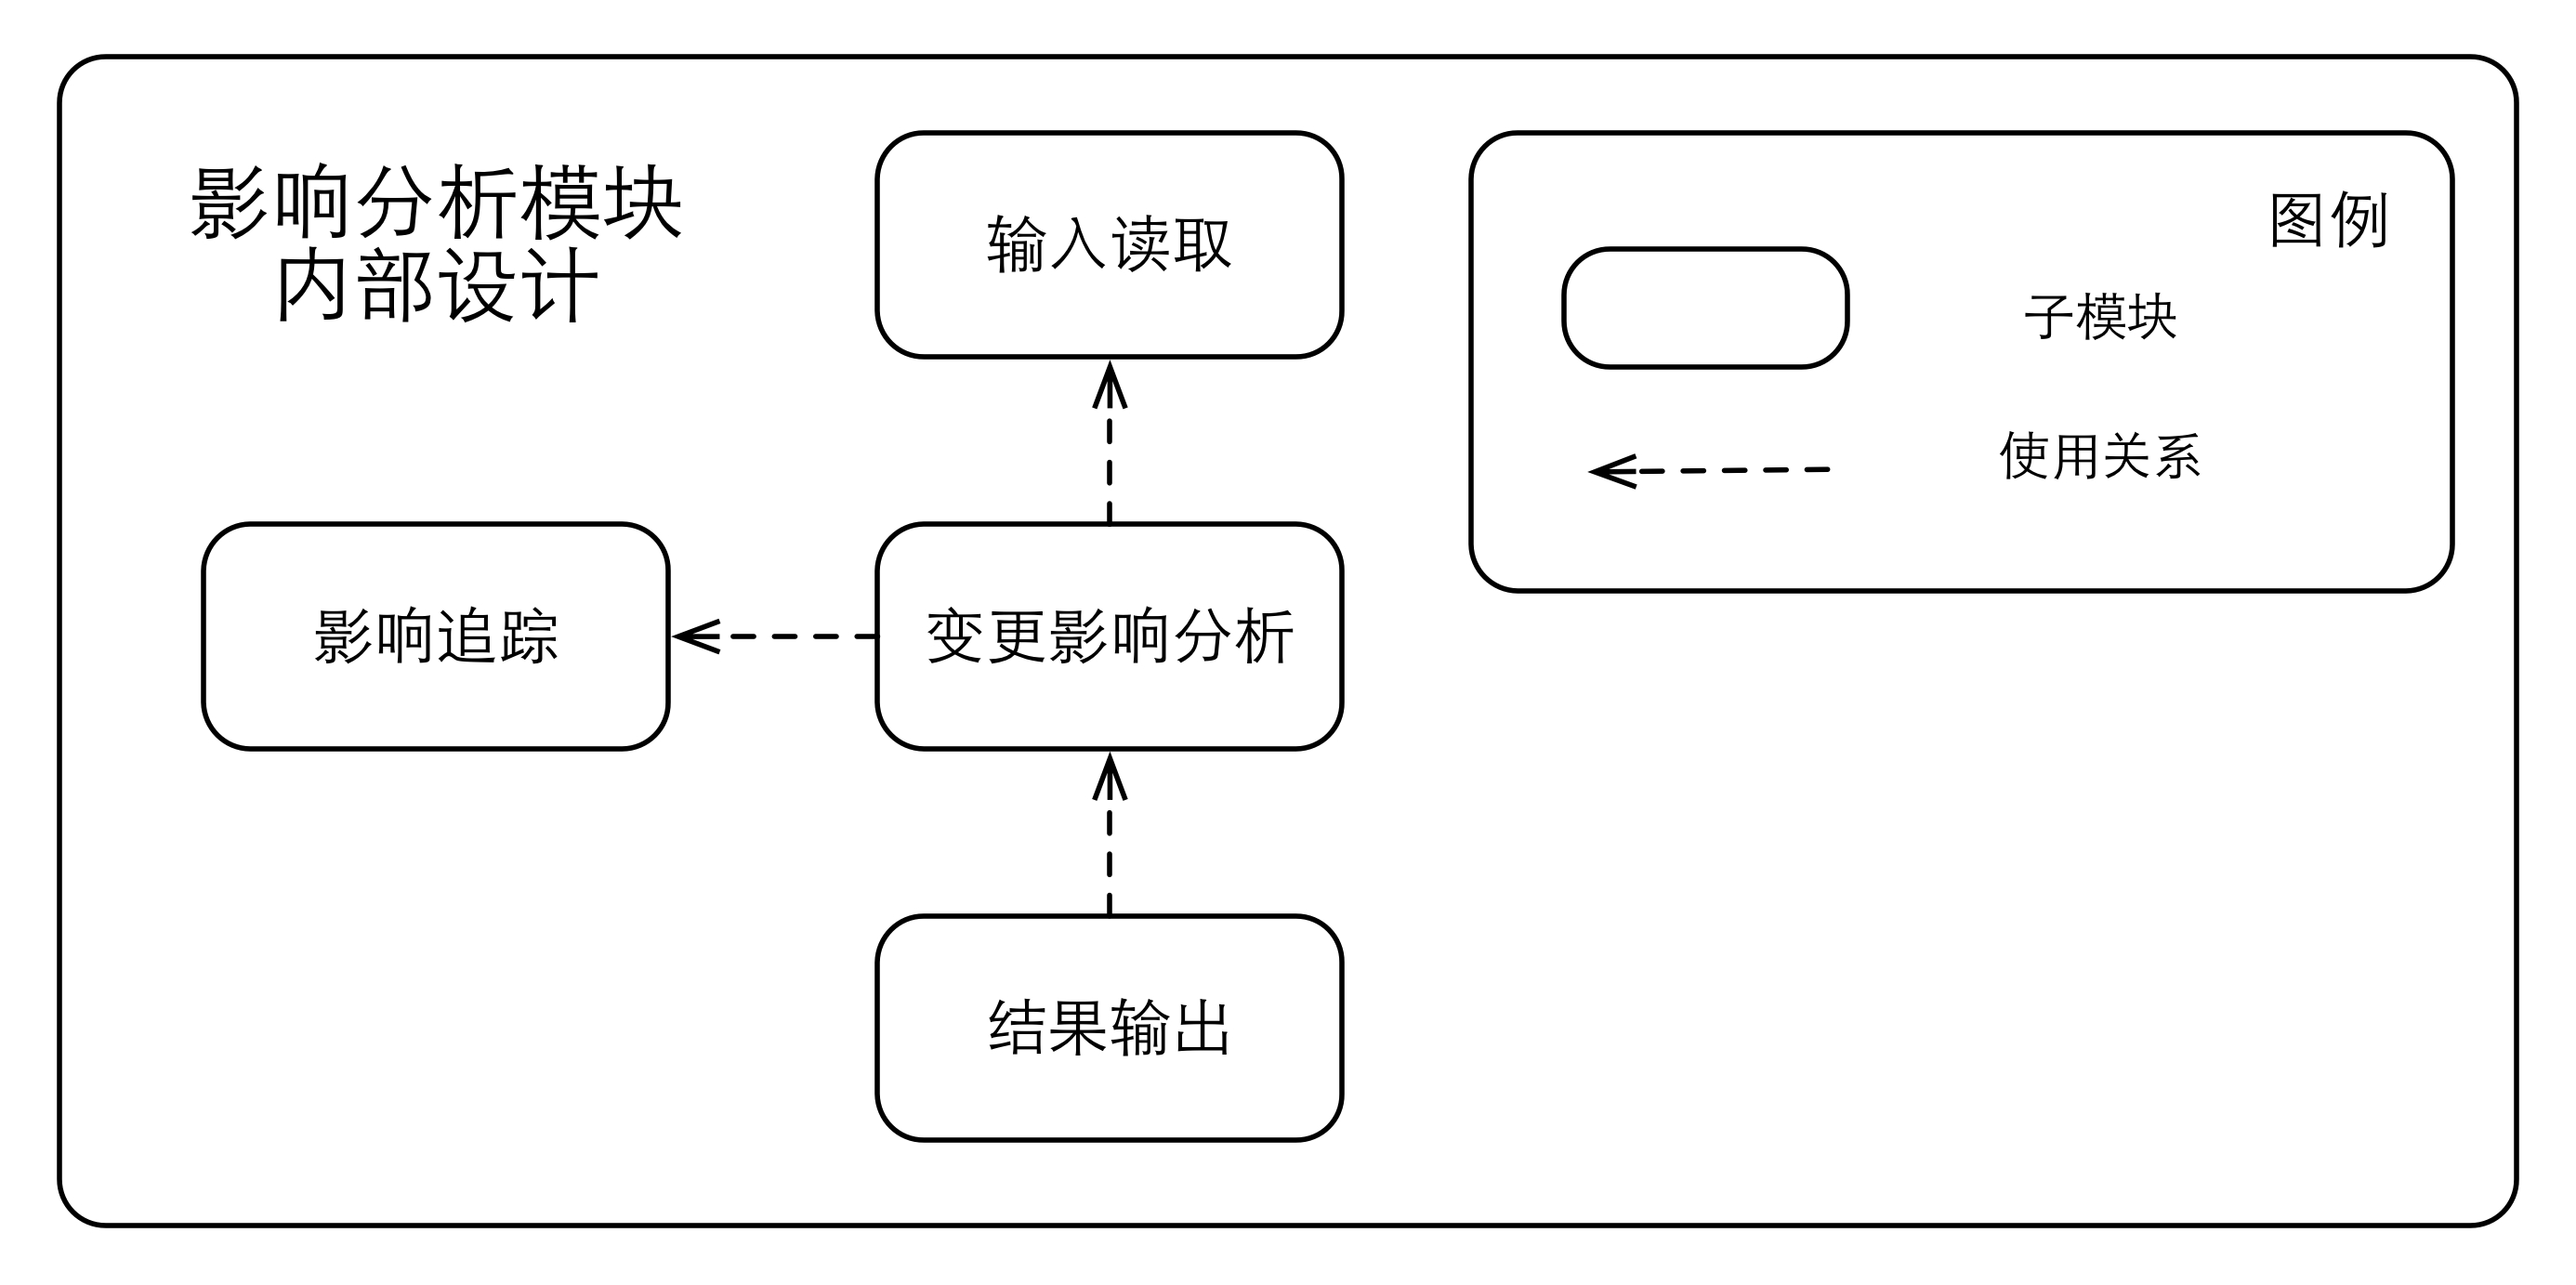
\includegraphics[width=.8\columnwidth]{chap04_impact_internal}
	\caption {模块设计}
	\label {des_impact}	
\end{figure}

\subsubsection{实现}


在本模块的实现中,实际上采用了jpf-regression来完成具体的影响分析工作。该工具接受Java格式的源代码作为输入,并输出Dot格式的影响域信息。

可见,该模块实际上是以Dot格式输出的影响域信息。Dot是一种采用文本进行描述的图形格式,以该格式输出的实际上是整个源代码的控制流图(Control Flow Graph),影响域作为该控制流图额外承载的信息,在CFG上进行了标注。

影响域的相关信息主要包括两类,
\begin{itemize}
	\item 受影响的CFG节点。这实际就是影响域中的元素。可见这里受影响元素的级别为基本块(Basic Block)。
	\item 影响的依赖关系。这实际是记录了受影响元素与影响来源元素之间的关系。该关系的定义可以参考章节\ref {define_problem}中所提到的$depend$映射关系。
\end{itemize}

该模块的实际输入输出可以参考表\ref {impact_io2}。

\begin{table}[H]
	\caption{输入输出对照表}
	\label{impact_io2}
	\centering
	\begin{tabular}{llc}
		\toprule[1.5pt]
		{\heiti 输入输出} & {\heiti 描述} & {\heiti 格式} \\\midrule[1pt]
		输入 & 差异性分析模块的输出,变更集合 & XML \\
		输入 & 源代码 & Java \\
		输入 & 源代码 & Class \\
		输入 & 配置文件 & JPF \\
		输出 & 语义影响域+控制流图 & Dot \\
		\bottomrule[1.5pt]
	\end{tabular}
\end{table}

jpf-regerssion是DiSE方法在Java Path Finder软件框架下的具体实现,提供了方法内和方法间的程序语句级别的变更影响分析。

然而jpf-regression工具中变更影响分析只是其中的一个子模块,主要用于为其后续的DiSE分析过程服务。因而在实践过程中,我们采用的解决办法是重用jpf-regression的代码,并对其加以改造,主要的变化包括:
\begin{enumerate}
	\item 修改分析流程。
	\item 增加影响追踪系统。
	\item 增加错误记录系统。
	\item 使其适应大规模批量化分析的需要。
	\item 已知Bug修复。
\end{enumerate}

下面分别进行介绍。


jpf-regression作为Java Path Finder框架的一个插件,事实上在使用时需要遵守该框架的约束,有明确的执行流程规定。然而在实际使用中,该流程约定与我们的实际情况并不合用,因而我们对此进行了一定的修正。

事实上,原执行流程约定,每次分析以源代码文件中的Main函数作为入口,探索并分析Main函数所调用的其他函数。该流程对于大部分情况而言是具有实际意义的,并且由于只考虑Main函数及其调用的函数,工具可以节约分析的开销,更快的得出结论,而忽略掉其他事实上并未在执行过程中被涉及到的函数。

然而对于我们的分析需要而言,该流程只能覆盖到部分情况,对于其他类型的软件系统而言可能并不适用,例如以Eclipse JDT Core项目而言,该项目主要用于为Eclipse软件系统的其他组件提供服务,因而在实际中以JAR包的形式作为库函数而存在。对于这类以库函数形式对外提供服务的源代码而言,他们并不存在入口函数,也无法预知到底会有哪些函数会被外界所调用。因而对于这类情况而言,我们需要在分析过程中覆盖其所有函数,以保证结果的完整性和正确性。

我们对于流程的修改可以参考图\ref {impact_process_old}进行对比。首先我们去掉了图\ref {impact_process}中所示的JPF框架启动流程,直接调用jpf-regression的核心功能。其次,如图\ref {impact_process_old}所示,我们将待计算的方法集合从Main函数的调用函数集合修改为文件中所有方法的集合,并在相应的影响集合计算过程中增加了影响追踪系统。

\begin{figure}[H]
	\centering
	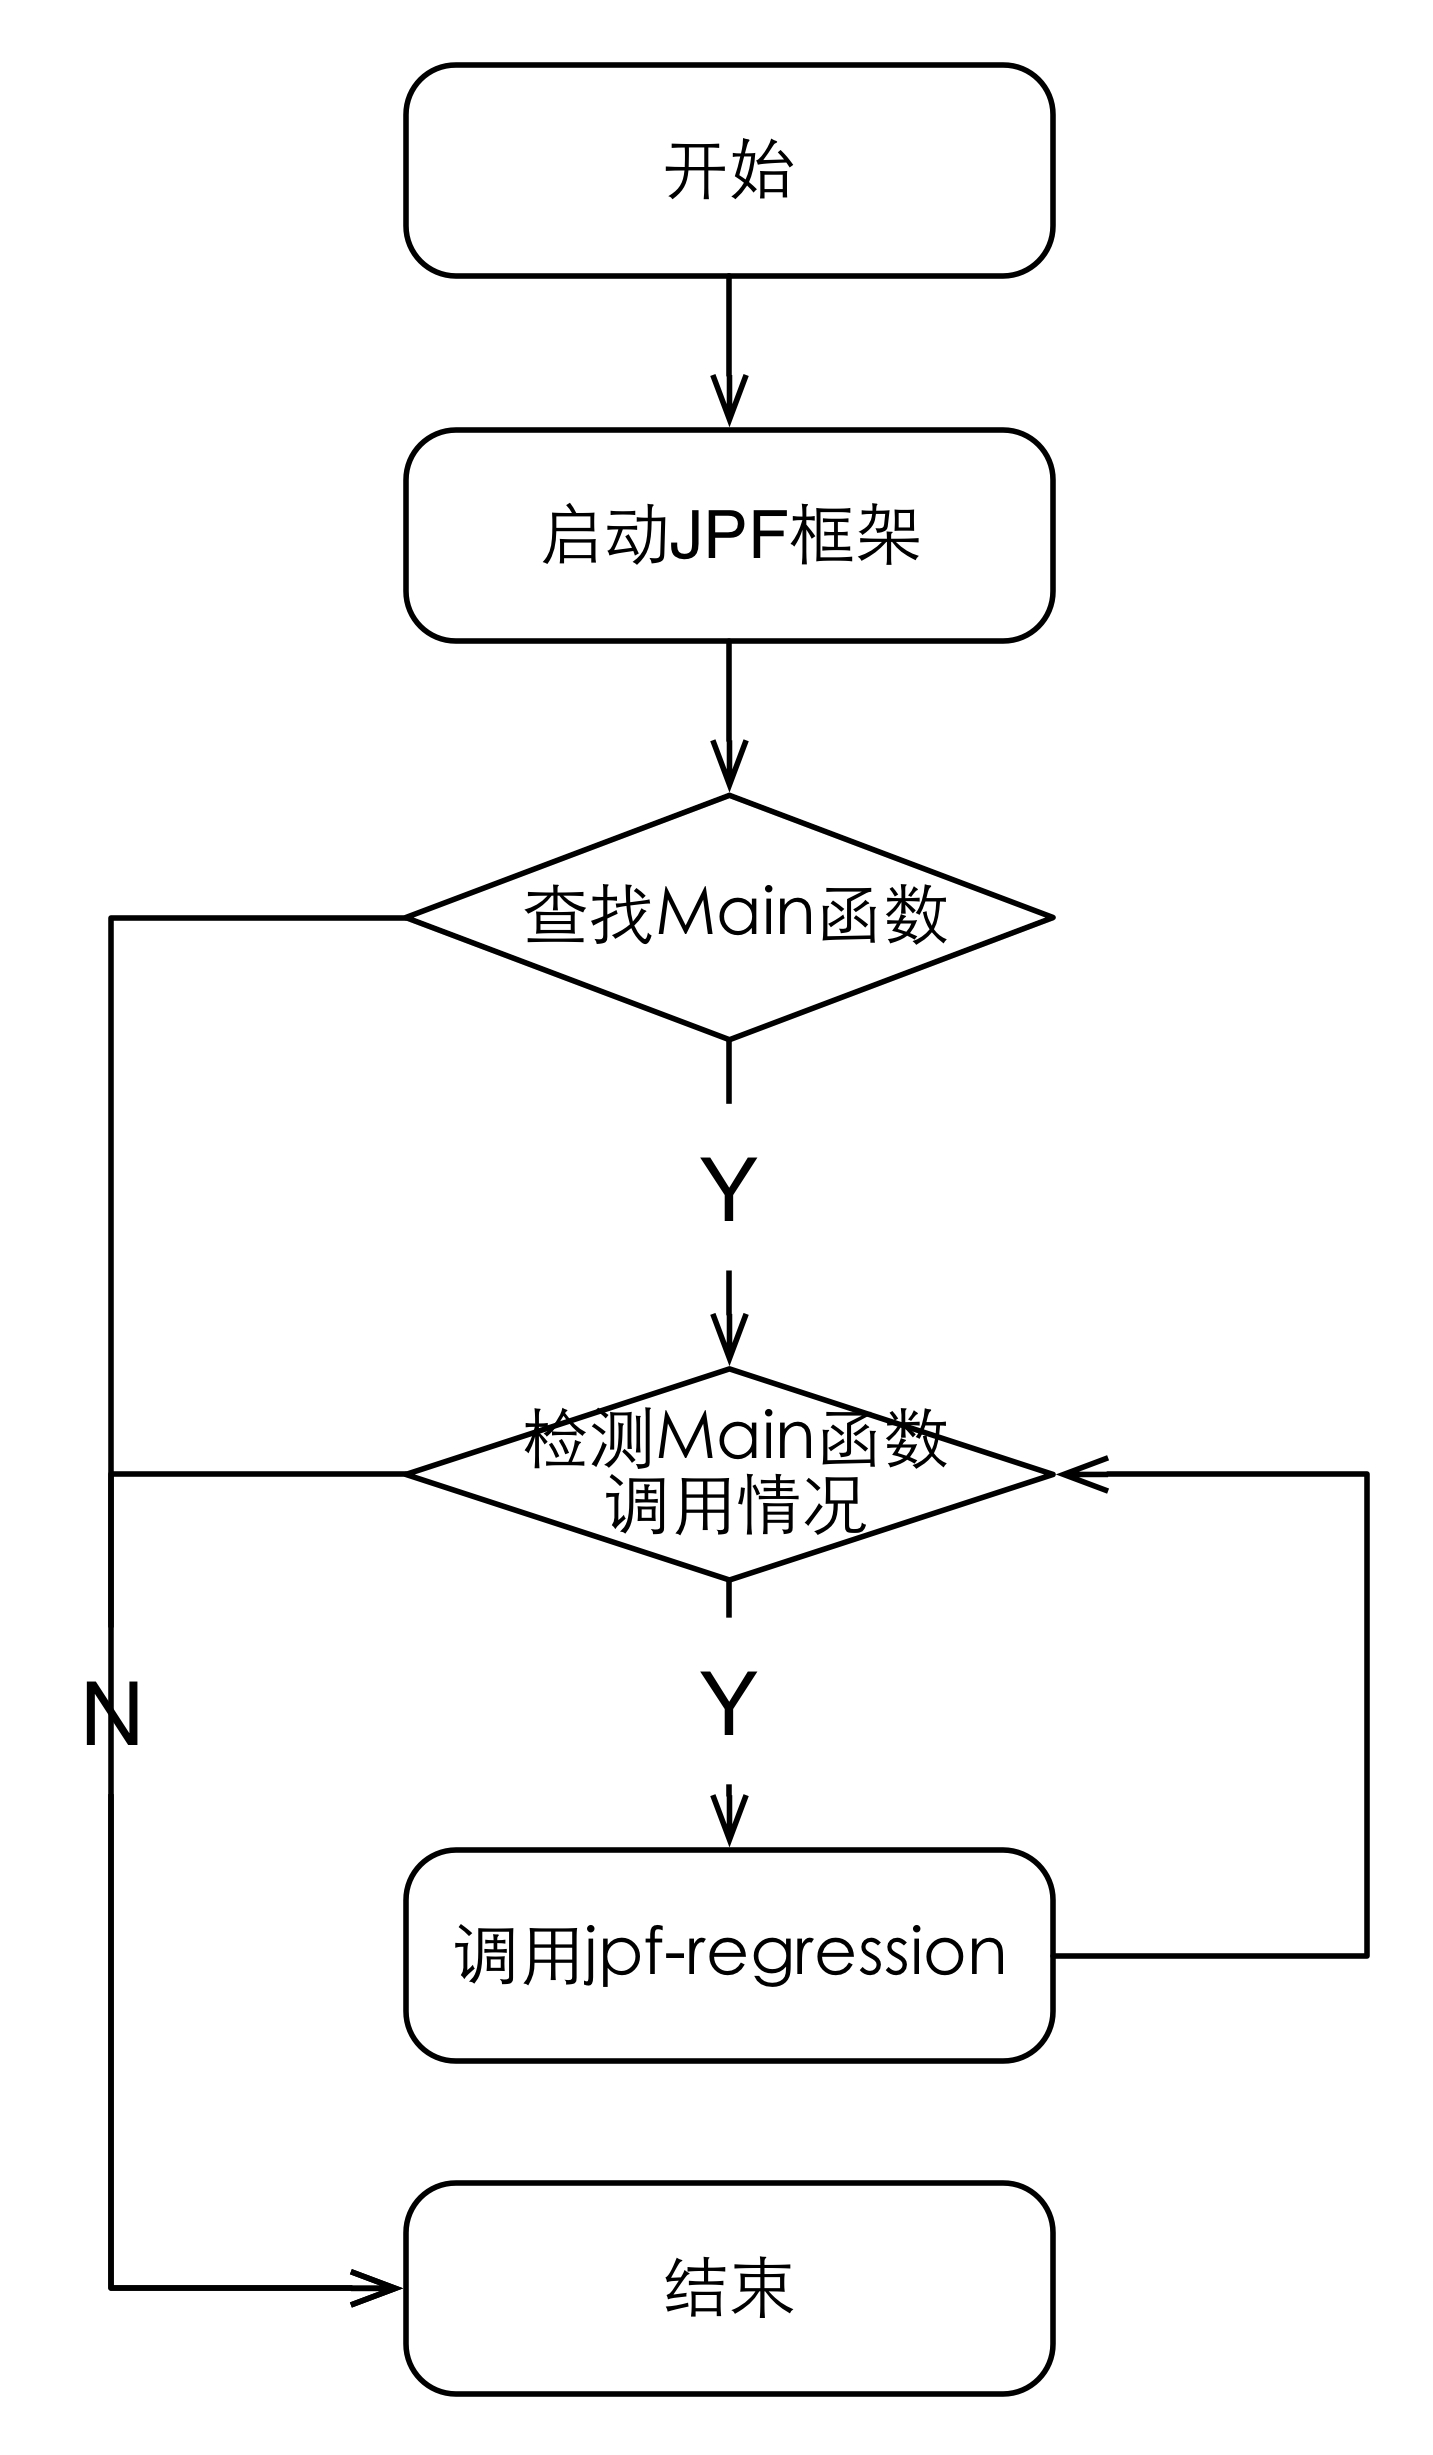
\includegraphics[height=.8\columnwidth]{chap04_jpf_launch}
	\caption {jpf框架启动流程}
	\label {impact_process}	
\end{figure}


\begin{figure}
	\centering
	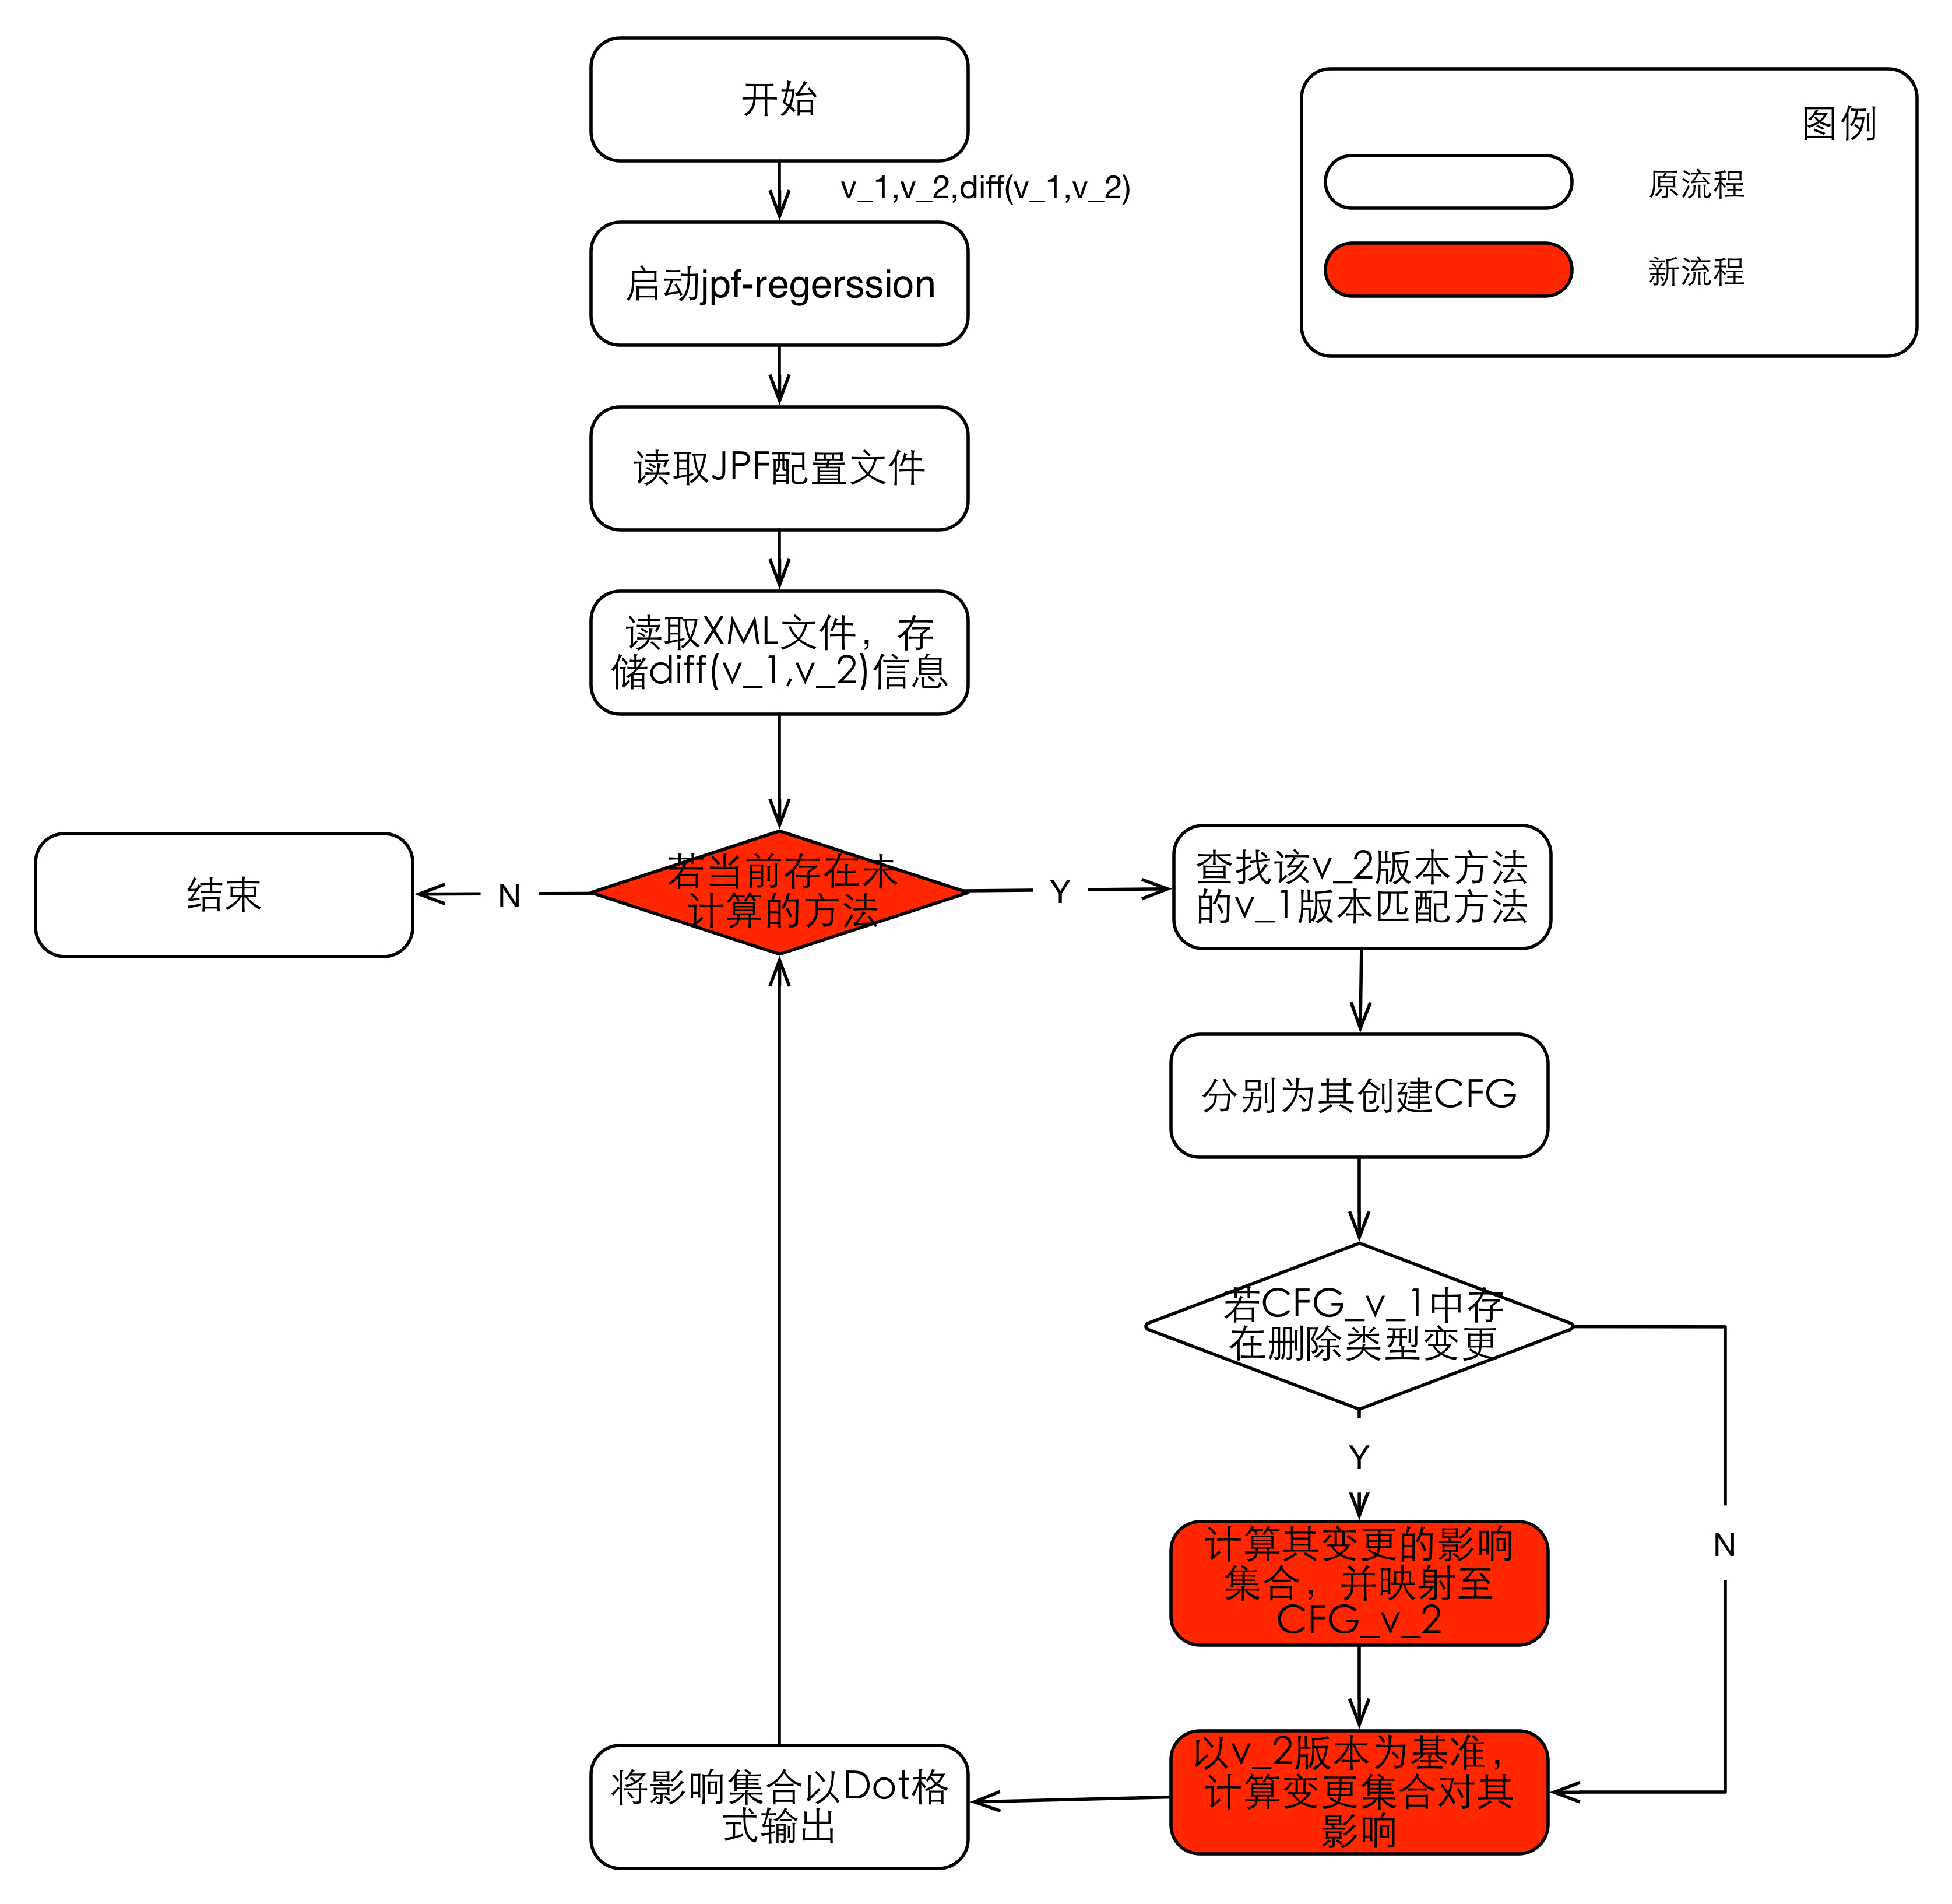
\includegraphics[width=.8\columnwidth]{chap04_jpf_old}
	\caption {jpf-regression原流程及变化}
	\label {impact_process_old}	
\end{figure}



在后续的冲突判定过程中,对于得到的冲突结果,我们需要对其追根溯源,挖掘其影响来源,以进行人工分析,判定该情况是否确实冲突。

因此,我们需要在变更影响分析的阶段加入影响追踪系统,以便记录下变更影响的轨迹,根据这些信息为后续的分析过程提供便利。

为了实现影响追踪系统,我们需要存储程序结构间的影响关系。如前所述,影响的来源主要有两类,即:
\begin{itemize}
	\item 控制依赖
	\item 数据依赖
\end{itemize}

因而,为了描述该影响依赖关系,本文设计了Dependency类族,参见图\ref {class_depend}。该类中使用了一个二元组的数据结构depend来存储影响来源和受影响对象,并使用了多态机制来区分影响关系的类型,即是控制依赖还是数据依赖。Dependency类族中重写了hashCode()方法和equals()方法,以便能够放入集合中进行存储。

影响追踪系统中具体使用到的数据结构可以参考表\ref {track_data}。

\begin{figure}[H]
	\centering
	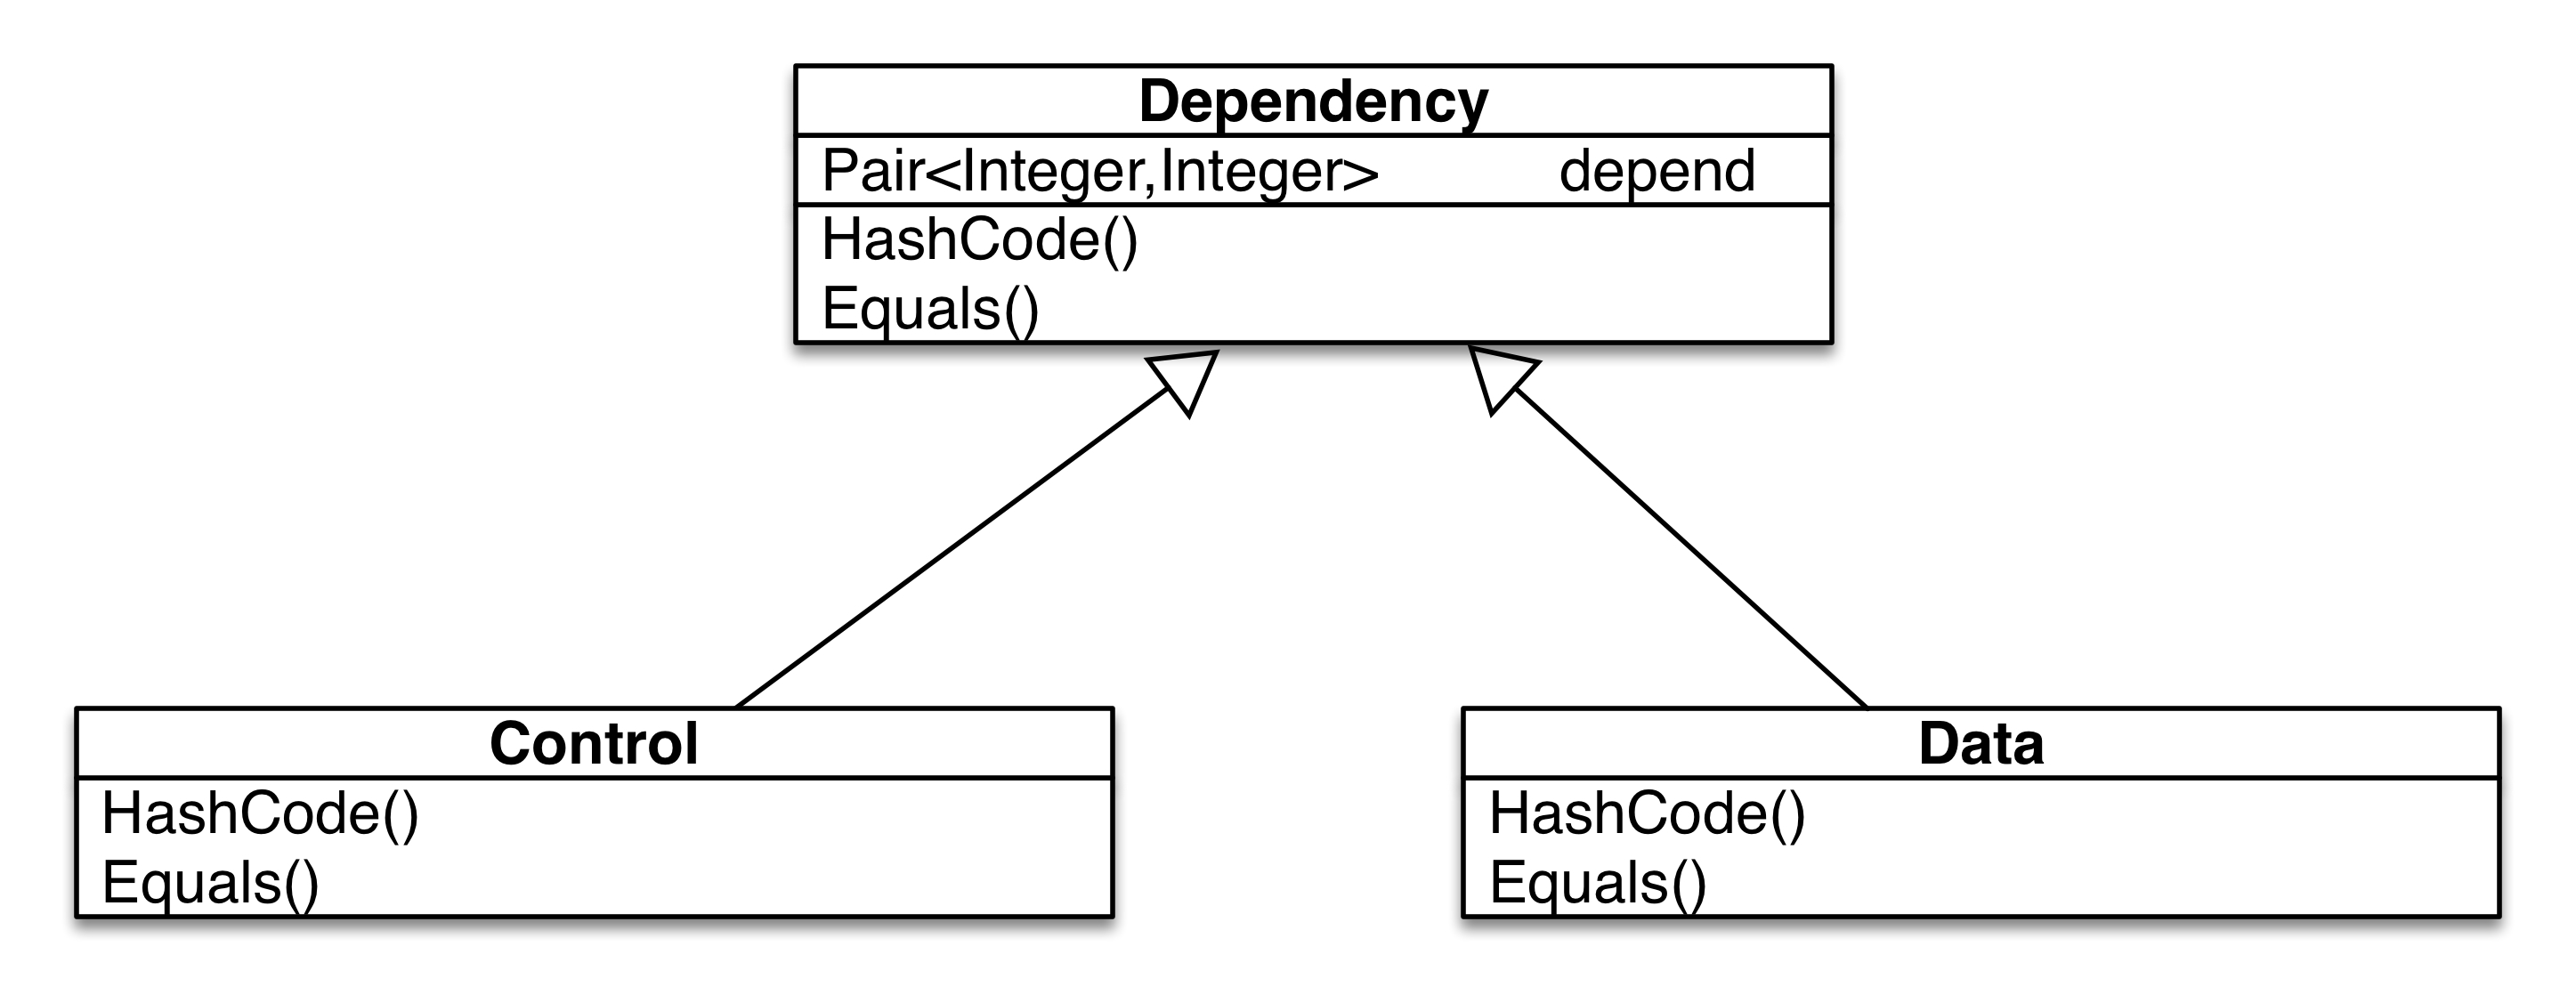
\includegraphics[width=.8\columnwidth]{chap04_depend}
	\caption {Dependency类族}
	\label {class_depend}	
\end{figure}

\begin{table}
	\caption{影响关系数据结构}
	\label{track_data}
	\centering
	\begin{tabular}{lllc}
		\toprule[1.5pt]
		{\heiti 数据类型} &{\heiti 数据结构} & {\heiti 用途} \\\midrule[1pt]
		Dependency & dependency & 单个影响关系 \\
		Control & dependency & 单个控制依赖影响关系 \\
		Data & dependency & 单个数据依赖影响关系 \\
		Map<Integer, Set<Dependency> > & depend & 存储计算过程中的全部影响关系\\
		\bottomrule[1.5pt]
	\end{tabular}
\end{table}

影响依赖关系的创建需要在进行变更影响分析过程的同时进行,以便记录下所有的依赖。最后将其输出到Dot文件中去,作为控制流承载的额外信息即可。

原有的jpf-regression工具由于是单次分析过程,因而一旦在运行过程中遇到问题,就会采用抛出异常终止运行的方式结束分析。然而我们在实际情况中需要进行大规模的分析作业,如果仅仅在其中单个文件的分析过程中出错就终止整个分析作业,会造成极大的时间和计算资源的浪费。

因而我们对该工具的异常处理方式进行了修改,使其在单次分析过程中如果遇到问题,则会及时抛出异常,但并不终止整个程序的运行,而采取了继续往下执行并分析其他文件的策略。然而分析错误是确实存在的,为了不丢失这类错误信息,我们为工具添加了错误记录系统,不断记录单次分析过程中遇到的问题。

我们对程序运行过程中可能出现的报错情况进行了分类,并设计了专门的错误统计类以专门别类的对错误情况进行记录和统计。该类的设计可以参考图\ref {class_error}。其中使用到的数据结构可以参考表\ref {error_data}的说明。

\begin{figure}[H]
	\centering
	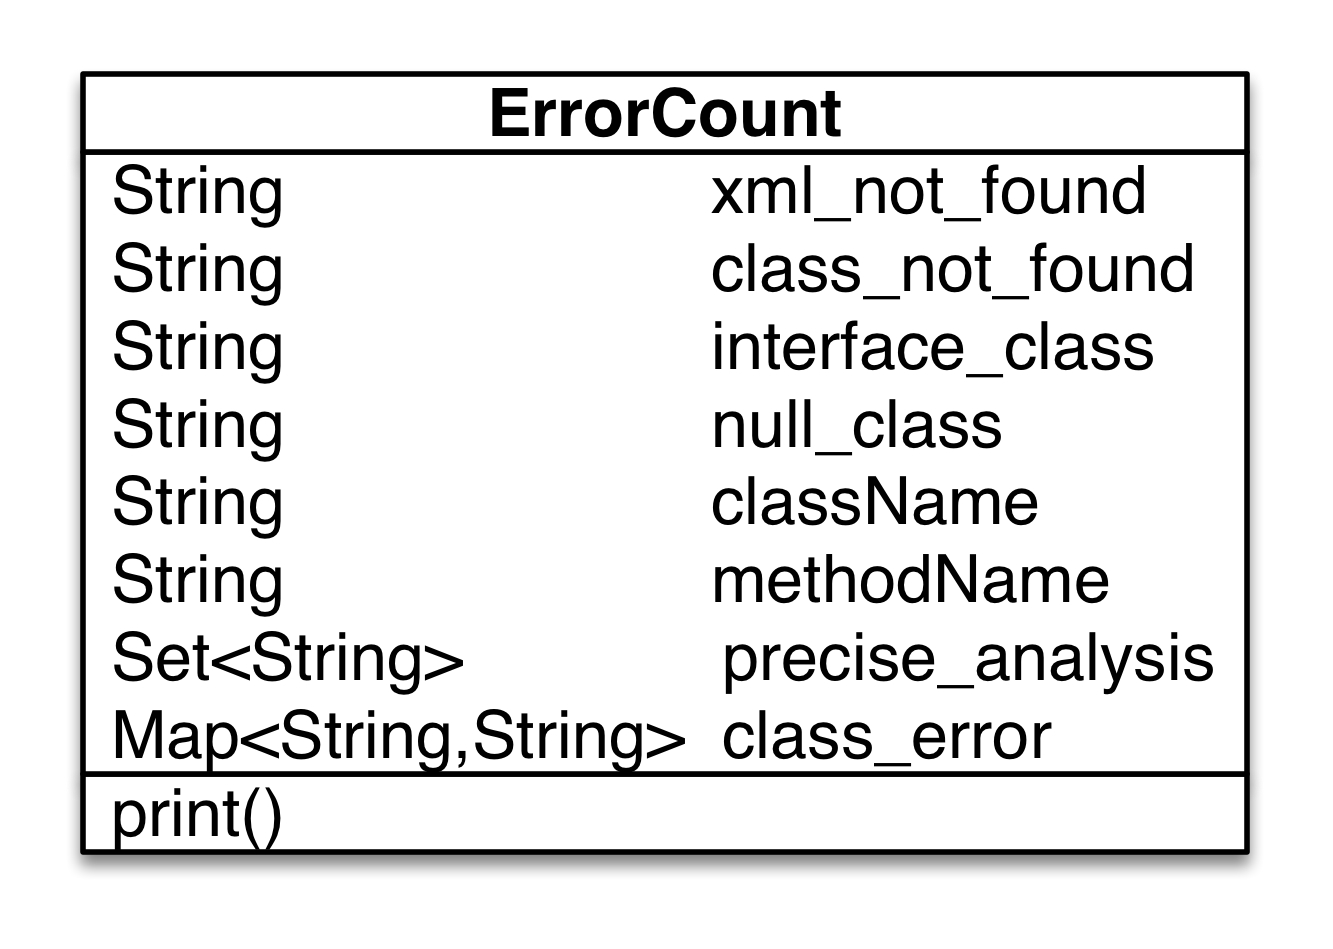
\includegraphics[width=.8\columnwidth]{chap04_error}
	\caption {ErrorCount类}
	\label {class_error}	
\end{figure}

\begin{table}
	\caption{错误记录数据结构}
	\label{error_data}
	\centering
	\begin{tabular}{lllc}
		\toprule[1.5pt]
		{\heiti 数据类型} &{\heiti 数据结构} & {\heiti 用途} \\\midrule[1pt]
		String & xml\_not\_found & 错误:XML文件未找到 \\
		String & class\_not\_found & 错误:Class文件未找到 \\
		String & interface\_class &  错误:接口类\\
		String & null\_class & 错误:类中无具体实现(如抽象类)\\
		Set<String> & precise\_analysis & 记录有多少方法在影响计算过程中出错\\
		Map<String, String> & class\_error & 记录有哪些类出现了哪些错误\\
		void & print() & 输出错误记录\\
		\bottomrule[1.5pt]
	\end{tabular}
\end{table}



原有的jpf-regression工具只能支持单次分析过程,在实际情况中我们需要工具具备大规模批量化分析的能力,以应对大规模软件系统的实际需求。为此我们可以保留原有的单次分析过程,然后在其上层进行封装,循环多次调用单次分析过程,以达到批量化自动分析的效果。这个过程由于进行了封装,对于用户而言是透明的。

同时,在进行大规模分析的时候,输出文件的命名格式也需要修改。在原单次分析过程中,输出文件直接采用被分析的方法名进行命名。对于分析小型文件而言,这种设计就足够了,然而在大规模分析的时候,我们需要进行一定的优化。

由于大规模分析时,可能存在一些现象,例如:
\begin{enumerate}
	\item 函数重载
	\item 不同版本间的代码其方法可能无法一一匹配。例如有的方法仅在单个版本的代码中出现。
\end{enumerate}

这些现象会使得工具中原有的输出文件命名方式不太合用。在这种情况下,我们采用的新命名格式为:

$MethodName+HashCode(MethodName)+ExtensionName$

其中,$MethodName$由即为方法名,无法保证方法名的唯一性。再利用Java中的HashCode方法,对$MethodName$计算其HashCode作为其后缀,以保证方法名的唯一性。最后$ExtentionName$即为文件扩展名,在jpf-regression中$ExtentionName = “.dot”$。

同时我们也保留了原有的单次分析能力,以满足实际情况中的其他需要,例如进行小规模的案例分析。

其次,在进行大规模分析的情况下,由于实验数据量的庞大,我们无法按照单次分析过程中那样去人工查看并分析实验结果。因此,为了适应这种需要,我们还增加了数据统计模块,使得程序具备一定的自动化分析实验结果的能力。

相关的类设计可以参考图\ref {class_run_all}和图\ref {class_run_jpf}。其中涉及的数据结构及其说明参考表\ref {run_all_data}和表\ref {run_jpf_data}。

\begin{figure}[H]
	\centering
	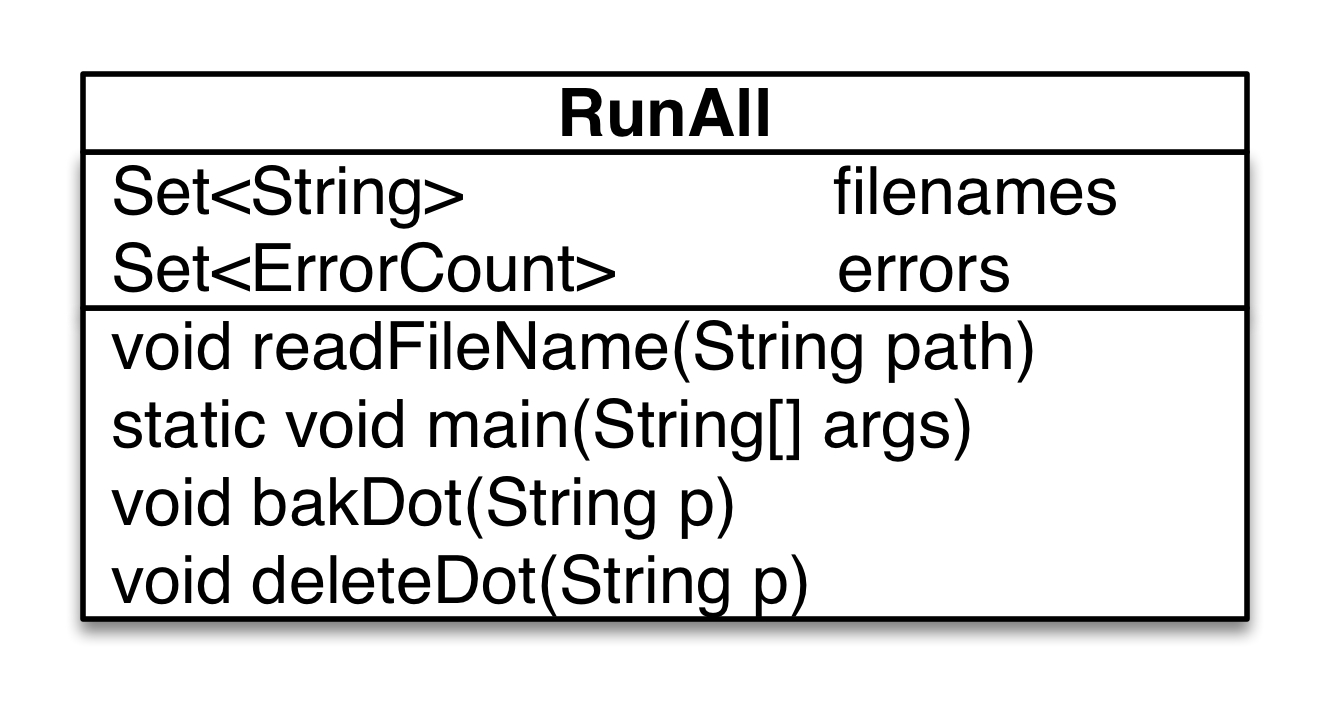
\includegraphics[width=.8\columnwidth]{chap04_run_all}
	\caption {RunAll类}
	\label {class_run_all}	
\end{figure}

\begin{figure}[H]
	\centering
	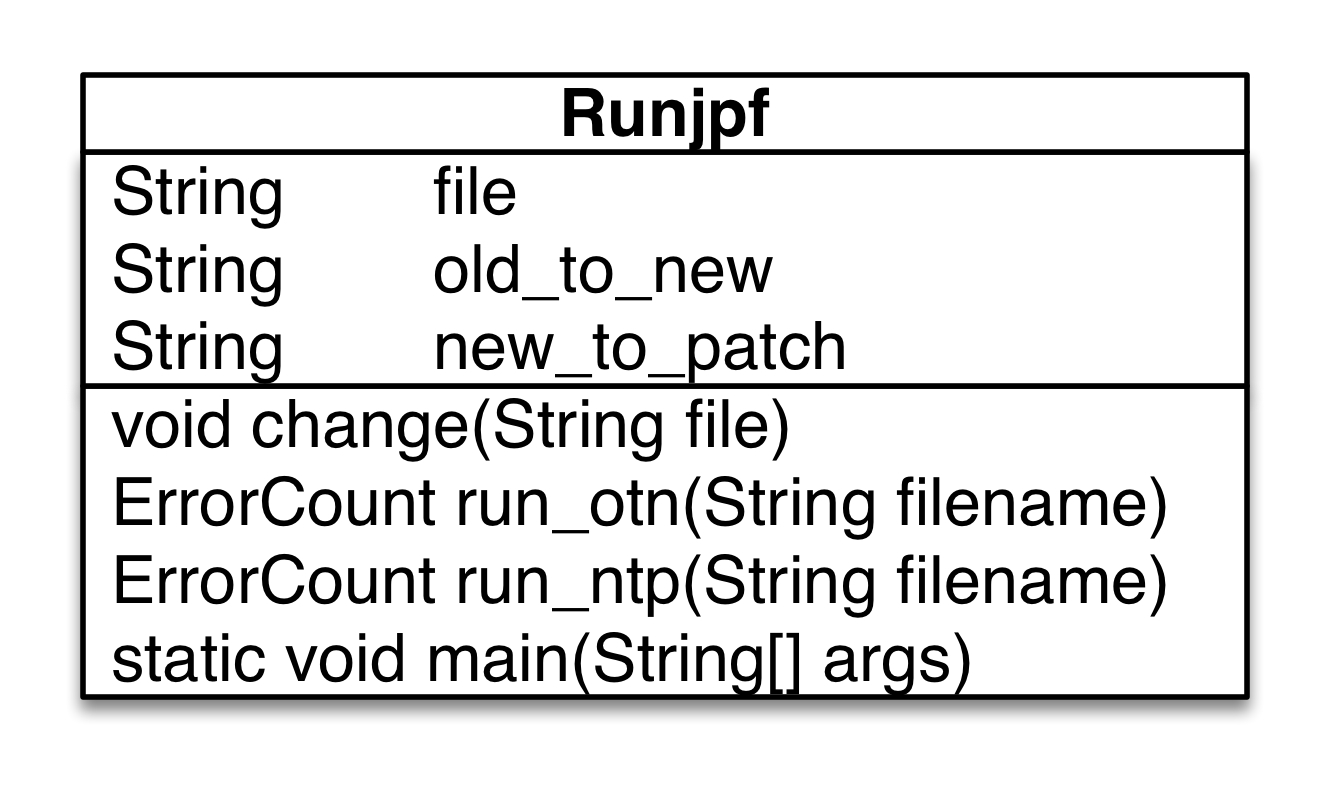
\includegraphics[width=.8\columnwidth]{chap04_run_jpf}
	\caption {Runjpf类}
	\label {class_run_jpf}	
\end{figure}

\begin{table}
	\caption{RunAll数据结构}
	\label{run_all_data}
	\centering
	\begin{tabular}{lllc}
		\toprule[1.5pt]
		{\heiti 数据类型} &{\heiti 数据结构} & {\heiti 用途} \\\midrule[1pt]
		Set<String> & filenames & 存储待分析的文件名 \\
		Set<ErrorCount> & errors & 存储每次分析中出现的错误 \\
		void & readFileName(String path) & 从文件中读取待分析的文件名\\
		static void & main(String[] args) & 实现大规模分析过程\\
		void & bakDot(String p) & 备份分析结果\\
		void & deleteDot(String p) & 删除分析结果\\
		\bottomrule[1.5pt]
	\end{tabular}
\end{table}

\begin{table}
	\caption{Runjpf数据结构}
	\label{run_jpf_data}
	\centering
	\begin{tabular}{lllc}
		\toprule[1.5pt]
		{\heiti 数据类型} &{\heiti 数据结构} & {\heiti 用途} \\\midrule[1pt]
		String & file & 待分析文件名\\
		String & old\_to\_new & $impact(diff(v_2,v_1),v_2)$过程的配置文件位置\\
		String & new\_to\_patch & $impact(diff(v_2,v_4),v_2)$过程的配置文件位置\\
		void & change(String file) & 改变当前需要读取的配置文件\\
		ErrorCount & run\_otn(String filename) & 运行$impact(diff(v_2,v_1),v_2)$过程 \\
		ErrorCount & run\_ntp(String filename) & 运行$impact(diff(v_2,v_4),v_2)$过程  \\
		static void & main(String[] args) & 实现单次分析过程\\
		\bottomrule[1.5pt]
	\end{tabular}
\end{table}


在实际使用jpf-regression进行实验的过程中,我们发现该工具存在一些Bug,这些Bug或多或少的导致了分析结果的正确性和精度降低。我们对其中力所能及的Bug进行了修复,并对这些Bug进行了总结。

目前已知的Bug及其修复情况可以参见表\ref {bug_data}。

\begin{table}
	\caption{Bug报告}
	\label{bug_data}
	\centering
	\begin{tabular}{lllc}
		\toprule[1.5pt]
		{\heiti Bug} &{\heiti 危害} & {\heiti 修复} \\\midrule[1pt]
		内部类无法进行方法匹配 & 小 & 否\\
		只有只有单个版本代码中存在某个方法时无法进行方法匹配 & 小 & 是\\
		将$CFG_{v\_1}$的影响集合映射到$CFG_{v\_2}$时判断条件出错 & 大 & 是\\
		依赖JAR包jpf\_guided\_test出错 & 小 & 否\\
		依赖JAR包jpf\_symboc出错 & 小 & 否\\
		\bottomrule[1.5pt]
	\end{tabular}
\end{table}

\section{本章小结}

本章中主要介绍了软件变更影响域分析方法和其对应的模块设计与实现过程。

章节\ref {chap_diff}中介绍了程序间差异性分析方法和其对应的模块设计与实现。

章节\ref {chap_impact}中介绍了变更影响分析方法和其对应的模块设计与实现。
